\documentclass[11pt,a4paper,twoside]{article}
\usepackage{bachelorarbeit}
\usepackage{subfigure}
\usepackage{xspace}
\usepackage{graphicx}
\usepackage[center]{caption}
\usepackage[english]{babel}
\usepackage{tikz}
\usepackage{caption}
\usepackage{float}
\usepackage{relsize}
\usepackage{stmaryrd}
\usepackage{latexsym}
\usepackage[justification=centering]{caption}

\setlength{\headheight}{52pt}
\setlength{\parindent}{0em} %Einrücken verhindern
\setcounter{tocdepth}{5}

% Zum Setzen von URLs
\usepackage{color}
\definecolor{darkred}{rgb}{.25,0,0}
\definecolor{darkgreen}{rgb}{0,.2,0}
\definecolor{darkmagenta}{rgb}{.2,0,.2}
\definecolor{darkcyan}{rgb}{0,.15,.15}
\usepackage[plainpages=false,bookmarks=true,bookmarksopen=true,colorlinks=true,
  linkcolor=darkred,citecolor=darkgreen,filecolor=darkmagenta,
  menucolor=darkred,urlcolor=darkcyan]{hyperref}

% Hier die eigenen Daten eintragen
\global\arbeit{Bachelor-Thesis}
\global\titel{Noninterference in the Take-Grant Model for the seL4 Microkernel}
\global\bearbeiter{Andrea Kuchar}
\global\betreuer{Dr Martin Hofmann, PD Dr Ulrich Sch\"opp}
\global\abgabetermin{07-27-2018}
\global\ort{Munich}
\global\fach{Computer Science}

\geometry{
  left=2.5cm,
  right=3.5cm,
  top=2.5cm,
  bottom=2.5cm,
}
\setcounter{secnumdepth}{5}

\pgfdeclareimage [ width =15 cm ]{RemoveGraphic1}{Pictures/RemoveGraphicOld/RemoveGraphic1}
\pgfdeclareimage [ width =14 cm ]{WriteGraphic1}{Pictures/WriteGraphicOld/WriteGraphic1}
\pgfdeclareimage [ width =15 cm ]{CreateUMO}{Pictures/CreateUMO/CreateUMO}
\pgfdeclareimage [ width =15 cm ]{CreateOther}{Pictures/CreateUMO/CreateOther}
\pgfdeclareimage [ width =15 cm ]{CreateOutside}{Pictures/CreateUMO/CreateOutside}
\pgfdeclareimage [ width =15 cm ]{OverviewObjects}{Pictures/OverviewObjects/OverviewObjectDomains2}
\pgfdeclareimage [ width =15 cm ]{GrantTCB}{Pictures/GrantTCB/GrantTCB}
\pgfdeclareimage [ width =15 cm ]{GrantOthers}{Pictures/GrantTCB/GrantOthers}
\pgfdeclareimage [ width =15 cm ]{GrantOutside}{Pictures/GrantTCB/GrantOutside}
\pgfdeclareimage [ width =15 cm ]{WriteTCB}{Pictures/WriteTCB/WriteTCB}
\pgfdeclareimage [ width =15 cm ]{WriteOthers}{Pictures/WriteTCB/WriteOthers}
\pgfdeclareimage [ width =15 cm ]{WriteOutside}{Pictures/WriteTCB/WriteOutside}
\pgfdeclareimage [ width =15 cm ]{WriteOutside2}{Pictures/WriteTCB/WriteOutside2}
\pgfdeclareimage [ width =15 cm ]{ReadTCB}{Pictures/ReadTCB/ReadTCB}
\pgfdeclareimage [ width =15 cm ]{ReadOthers}{Pictures/ReadTCB/ReadOthers}
\pgfdeclareimage [ width =15 cm ]{ReadOutside}{Pictures/ReadTCB/ReadOutside}
\pgfdeclareimage [ width =15 cm ]{ReadOutside2}{Pictures/ReadTCB/ReadOutside2}
\pgfdeclareimage [ width =15 cm ]{RemoveCNode}{Pictures/RemoveCNode/RemoveCNode}
\pgfdeclareimage [ width =15 cm ]{RemoveOthers}{Pictures/RemoveCNode/RemoveOthers}
\pgfdeclareimage [ width =15 cm ]{RemoveOutside}{Pictures/RemoveCNode/RemoveOutside}
\pgfdeclareimage [ width =15 cm ]{RemoveOutside2}{Pictures/RemoveCNode/RemoveOutside2}
\pgfdeclareimage [ width =15 cm ]{RevokeCNode}{Pictures/RevokeCNode/RevokeCNode}
\pgfdeclareimage [ width =15 cm ]{RevokeOthers}{Pictures/RevokeCNode/RevokeOthers}
\pgfdeclareimage [ width =15 cm ]{RevokeOutside}{Pictures/RevokeCNode/RevokeOutside}
\pgfdeclareimage [ width =15 cm ]{RevokeOutside2}{Pictures/RevokeCNode/RevokeOutside2}

\begin{document}
	
% Cover
\deckblatt
	
	
% Declaration of authorship
\declaration
\pagenumbering{Roman}
\selectlanguage{english}

% Abstract
\clearpage
\section*{Abstract}
\addcontentsline{toc}{section}{Abstract}
	
The thesis investigates the question whether the specification of the seL4 access control system is strong enough to verify Noninterference properties on it. I analyse the Take-Grant-Protection Model \cite{TakeG} and extend it for showing the Noninterference properties \cite{InfFlow} on each of its system operations. 
As the specifications and proofs of the take-grant model are developed in the theorem proof assistant Isabelle/HOL, I use the same to formalise my datatypes and functions. 
	

\newpage
%Abbildungsverzeichnis
\listoffigures
\newpage
% tableofcontents
\tableofcontents

	
\clearpage
% Hier beginnt der eigentliche Text
% !TEX root = Bachelorarbeit.tex
\chapter{Introduction}
	\pagenumbering{arabic}
	\section{Motivation}
Nowadays our society becomes progressivly dependent on computer systems.\\ Througout our whole life smaller and smaller computers increasingly take over control. Wheter in a smart TV, our car or the lights in a connected home. We are therefore forced to confront ourselves with the safety and reliability of these systems. \\
This is particular essential when we entrust our lives to one of these computers. We expect on-board computers in cars or flight-computers to be free from defects and unhackable. Unfortunately the reality is often different. For example, hackers have proven that the onboard computer of some cars can be taken over from a smartphone in a nearby car. \\
A key component in developing secure systems is the operating-system (OS) kernel. The kernel has full access to hardware resources. One defect in the kernel can compromise the security and reliability of the entire system. \\
The weakness of most traditional kernels was their huge amount of code due to their monolithic design. This makes it hard to review or verify the code. Monolithic designs are fundamentally week because they integrate accessory functions like drivers for hardware or virtual filesystems. This makes the system more vulnerable for bugs. One crashed module can lead to a crash of the entire system. \\
In contrast, microkernels concentrate on the fundamental functions: interprocess communication, scheduling or memory management. The motivation behind microkernels is to reduce the  possibility of bugs in the kernel code through reducing the code to an amount as minimal as possible and to exclude functions from kernel mode. With less code it becomes more feasible to guarantee the absence of defects within the kernel through formal verification.\\
Because we feed our smartphones, tablets, on-board computers, etc. with an ever growing amount of sensitive information like bank data, passwords, e-mails, chats the safety of embedded systems is a growing necessity. \\
Through isolation of small subsystems, like it is done in microkernels, the security already can be raised to a higher level. With testing one can detect an huge amount of bugs. But as Dijkstra said "Testing can only show the presence, not the absence, of bugs." \cite{EngTec} \\
As already mentioned, less lines of codes makes it more feasible to verify it relating to its specification. 
The seL4 microkernel is the first microkernel whose correctness is formally verified. It is a high-assurance, high-performance microkernel, primarily developed, maintained and formally verified by NICTA (now Trustworthy Systems Group at Data61) for secure embedded systems. Its security model is based on the take-grant model, which was extended for being able to reason about kernel memory consumption of components. 
	\section{Aim of the thesis}
	With this thesis I will explore if the extended take-grant model is strong enough to show noninterference properties on it. \\
	The security property of noninterference ensures that there is no unwanted information flow within a system. The take-grant model is an access control model. Therefore its duty is to "control" the access or the transfer of access on objects of a system. The noninterference property assures that there is no way information can flow to undesirable parties. \\
The thesis should investigate the different system operations of the model regarding the thereby occurring information flow. \\
With the collected information I want to answer two questions. First if the noninterference properties can be illustrated on the existing take-grant model and second if the noninterference properties are fulfilled or the different system operations the take-grant model provides. 
\section{Structure of the Thesis}
At the beginning I want to give a survey of the seL4 kernel, its set-up, the implementation of services and the memory management. For a better comprehension I then give a brief overview of the take-grant and the noninterference model. 
Chapter 3 focuses on the formalisation of the take-grant model an Chapter 4 on the formalisation of the noninterference model. \\
From chapter 5 on I turn to the validation of the noninterference property. In chapter 7 the validation is subdivided into the different system operations. To show the property for the model I am going to extend the model in Chapter 6. \\
Finally I'll take a short resume and give a prospect on the possibilities to enhance this topic.
	 
\newpage
\section{Requirements}
% !TEX root = Bachelorarbeit.tex
\subsection{The seL4 Microkernel}\label{sec:seL4}
	The seL4 \cite{Manual} ist a small operation system kernel developed for the ARM11 arcitecture. All concepts, however, can be generalised to any architecture with a multilevel-page-table structure. \cite{PhDseL4} It is based on the L4 microkernel developed in the 1990s and proviedes a minimal number of services to applications, such as abstractions for virutal address spaces, threads, inter process comunication (IPC). \\
	Each abstraction ist implemented by a kernel object with methods dependent on the abstraction it supplies. If an application whants to use one of the implemented services it to call the corresponding object through capabilities. They are stored in kernel objects called \textit{CNodes}. \\
	Each capability contains a target object and potentially several access rights. The access rights can be \texttt{Read, Write, Grant} and \texttt{Create}. By invoking a capability that points to the kernel object  with a corresponding method name, applications can invoke system calls. As arguments these system calls can have data or other capabilities. For example: If an object has a capability with write authority in it, pointing on a synchronous endpoint, it can send a message to another object, that has read authority on this endboint. It can do it by invoking the capability, with the write right in it, that points on the synchronous endpoint object. The other object in turn has to own and invoke a capability with the read right in it, that also point on the synchronous endpoint.

\subsubsection{System Calls}
The kernel provides the following system calls:
\begin{itemize}
\item \texttt{send()}: The system call argument is delivered to the target object and the application is allowed to continue. If the target is not able to receive and/or process the arguments immediately, the sending application will be blocked until the arguments can be delivered.

\item \texttt{NBSend()}: Like \texttt{send()}. Exception: If the message is not deliverable it is silently droped.
\item \texttt{Call()}: Like \texttt{send()} but the application is blocked until the object provides a response, or the receiving application replies. \\
If the argument is delivered to an application via Endpoint the receiver needs the right to respond to the sender. So in this case an additional capability is added to the arguments. 
\item \texttt{Wait()}: If the target object is not ready \texttt{Wait()} is used by an application to block until the object is ready. 
\item \texttt{Reply()}: Used to respond to a \texttt{Call()}, using the capability generated by the \texttt{Call()} operation.
\item \texttt{ReplyWait()}: As a combination of \texttt{Reply()} and \texttt{Wait()} it is efficent for the common case that replying to a request and waiting for the next can be performed in a single system call. 
\end{itemize}
	
\subsubsection{Kernel Objects}\label{sec:KernelObjects}
The kernel implements several objects to allocate the system operations \cite{Manual}.
\begin{itemize}
\item \textbf{CNodes} \\
The capabilities to invoke system calls are stored in \textbf{\textit{CNodes}}. When created they get a fixed numer of slots that can be empty or contain a capability. 
The kernel constructs a \textbf{Capability Derivation Tree} (CDT) to keep records about the created capabilities and their associations. This is required for the revoke operation. \\ 
They have the following operations:
\begin{itemize}
\item \texttt{Mint()} \\
creates a copy of an existing capability. The new capability is placed in a specified CNode slot and may have less rights than the parent capability. In the CDT the capability is placed as child of the original one. 
\item \texttt{Copy()} \\
is similar to the Mint operation. But the new capability has the same rights as the original one and in the CDT it is represented as a sibling of it. 
\item \texttt{Move()} \\
can move a capability between two specified slots. 
\item \texttt{Mutate()} \\
moves the capability similar to \texttt{Move()} and is able to reduce its rights as it is done in \texttt{Mint()} without an orignal copy remaining.
\item \texttt{Rotate()} \\
moves two capabilities between three slots. Replaces two \texttt{Move()} operations. 
\item \texttt{Delete()} \\
can remove a capability from a specified slot.
\item \texttt{Revoke()} \\
is used to remove a complete part of the CDT. From a defined capability on, all children from the capability in the CDT are removed with \texttt{Delete()}. 
\item \texttt{Recycle()} \\
revokes all outstanding capabilities and reconfigures the object to its initial state. So the object can be reused in for another purpose.
\end{itemize}

\item \textbf{IPC Endpoints} \\
Endpoints are used for the \textit{interprocess communication} between threads. They can be devided into \textbf{synchronous (EP)} and \textbf{asynchronous (AEP)} endpoints. 
Threads in the seL4 kernel are grouped into security domains. Interprocess communication between different domains is only realised via AEPs. Generally capabilities to endpoints can be restricted to be read - or write - only. 
\item \textbf{TCP} \\
A thread of execution in seL4 is represented by a \textit{thread control block}. It is always associated with a CSpace (provides the capabilities required to manipulate the kernel objects) and a VSpace (provides the virtual memory environment required to contain the code and data application). \\
The thread control block object has the following methods: \\
\texttt{CopyRegisters(), ReadRegisters(), WriteRegisters(), SetPriority(), \\ SetIPCBuffer(), SetSpace(), Configure(), Suspend(), Resume()}
\item \textbf{Virtual Memory}\\
In the \textit{virtual address space} (VSpace) Objects in the VSpace implement services for the management of virtual memory which largely directly correspond to those of the hardware: \\
\begin{itemize}
\item seL4 ASID Table: \\
The seL4 \textit{Adress Space Identifier} table provides two services:
\begin{enumerate}
\item With the seL4 ASID table address spaces where mappings have to be removed from can easily be detected, as the seL4 acts as an internal naming mechanism for them.
\item In the seL4 PageDirectorys can be deleted without updating the capability links because the kernel sets the corresponding PageDirectory address in the ASID table to \textit{NULL} if a PageDirectory is revoked. Therefore the seL4 ASID table provied so called \textit{weak links} between capabilities on addresses in the ASID table and the VSpace mappings that are derived from them.
\end{enumerate}
The seL4 ASID table is a global, fixed-sized table that is created at boot time. Each seL4 ASID is associated with a hardware ASID.
\item PageDirectory (PD): \\
It defines the root page table of the two-level , hardware defined page table structure the ARM11 consists of. If an entity owns a authorised capability that points to a PD it has the right to manipulate the related VSpace.
\item PageTable (PT): \\
The leaf node of the ARM11, two-level page table structure is implemented by the PageTable object. A page table entry contains either an invalid
entry, or a pointer to a 4 kilobyte Page.
\item Pages or Frames: \\
A virtual memory page is implemented by region of physical memory called a \textit{Page} or \textit{Frame}. The name differs from paper to paper. In the specification it is called a \textit{Page} \cite{sel4}. It has three methods:
\begin{itemize}
\item If it gets an PD or PT capability as an argument the \texttt{map} installs a PD-entry or PT-entry and refers to the Page in the specified location.
\item If the permissions of an existing mapping have to be changed the Page calls the \texttt{remap} method.
\item The \texttt{unmap} method is used to remove an existing mapping.
\end{itemize}
\end{itemize}
The following illustrates the creation of a VSpace:
\begin{enumerate}
\item First a PD object has to be allocated with the retype operation on untyped memory objects. 
\item The \textit{Resource Manager} has to initialise it with a seL4 ASID table:
\begin{itemize}
\item It invokes the PD object
\item It passes a capability that allows the use of a slot in the seL4 ASID table. The memory address of the PD is copied into the provided ASID table slot. 
\item The capability pinting on the PD is updated by storing the sel4 ASID table index into it instead of the PD index. 
\end{itemize}
\item Now the PD can be used as a VSpace of one or more threads.
\item The ressource manager can install a PageTable into  an adress space by invoking a PageDirectory and passing a PageTable capability and the virtual address. After installing a PageTable the kernle stores the seL4 AID of the corresponding PD and the virtual address in the PT capability. 
\item With Pages the kernel proceed in a similar way. 
\end{enumerate}
Figure \ref{fig:intapp} shows how the objects of a VSpace are connected.
\begin{figure}[H]
	\centering
		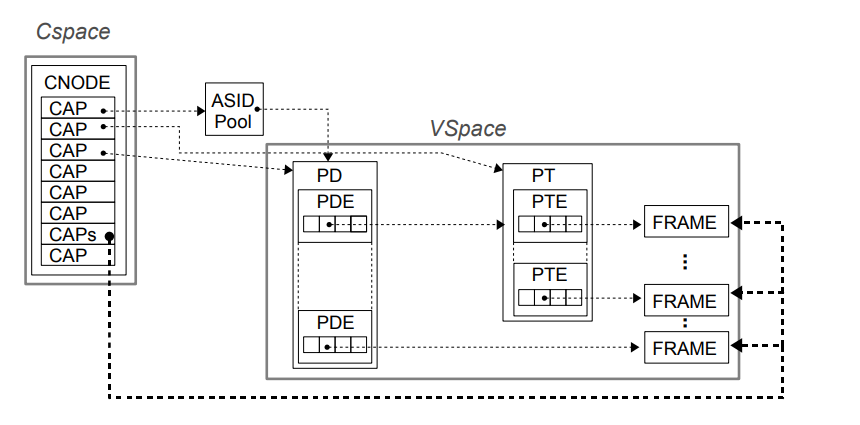
\includegraphics[width=0.7\textwidth]{./Pictures/applicationIntern.png}
	\caption[Internal representation of an application]{Internal representation of an application in seL4 \cite{sel4}}
	\label{fig:intapp}
\end{figure}
\item \textbf{Interrupt Objects} \\
Device driver applications require \texttt{Interrupt Ojects} to be capable of receiving and acknowledging interrupts from hardware devices.
\item \textbf{Untyped Memory} \\
\texttt{Untyped memory objects (UMO)} encapsulate a fixed-sized, size-aligned, continuous region of the physical memory. Each object can be devided into a group of smaller untyped memory objects. With \texttt{Retype()} a number of new kernel objects are created. It also returns capabilities to the new objects if it succeeds. 
\end{itemize}

\subsubsection{Memory Allocation Model} 
A special characteristic of the seL4 is that the memory for kernel objects is not allocated dynamically. A goal was to isolate physical memory access between applications and to control the amount of physical memory that applications can use. \\
To accomplish this applications get fixed sized memory regions they have to control by themselves. \\
Capabilities on Untyped Memory Objects (UMO) are needed to create new objects. So applications need the capabilities on UMOs to create new objects. After creation the objects have a fixed amount of memory they can use. \\
At boot time the kernel pre-allocates all the memory required for the kernel to run. This includes the space for kernel code, data and kernel stack. The kernel then creates an \textit{Initial User Thread} with associated CSpace and VSpace and hands over the remainig memory in form of capabilities on UMOs. \\
The Initial User Thread can create smaller sized UMOs out of an UMO or \texttt{retype} it into another object type. The creator of new objects has full authority over the objects. This "full authority" depends on the object type. \\
Figure \ref{fig:systarch} shows a sample system architecture in which a resource manager running at user-level  has the authority over the remaining untyped memory after bootstrapping. 
	
	\begin{figure}[ht]
	\centering
		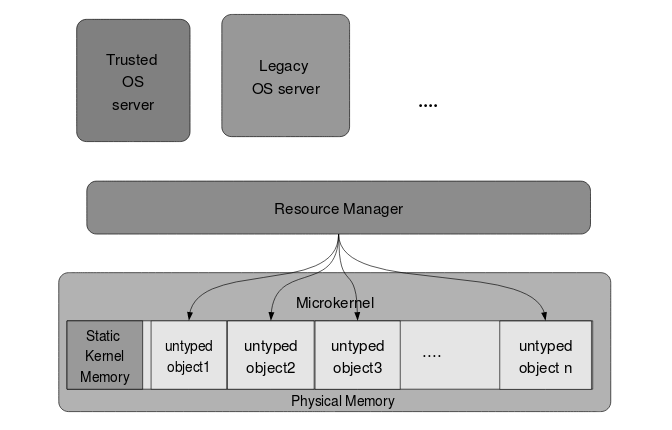
\includegraphics[width=0.6\textwidth]{./Pictures/MemoryAllocation.png}
	\caption[Sample system architecture]{Sample system configuration \cite{TakeG}}
	\label{fig:systarch}
	\end{figure}	
\newpage
% !TEX root = Bachelorarbeit.tex
\subsection{The Take-Grant Model}	
Protection or acces control models specify, analyse and implemente security policies. 
The classical Take-Grant Model was primary introduced by Lipton and Snyder, 1977 in  \href{https://www.cs.nmt.edu/~doshin/t/s06/cs589/pub/2.JLS-TG.pdf}{%
"A Linear Time Algorithm for Deciding Subject Security"} \cite{1TG}.
\subsubsection{The Classical Model}
In the Take-Grant Model \cite{TakeG} subjects or objects are represented as nodes and authority as arcs in a directed graph that represents the system. \\ 
Rules for graph mutation represent the different system operations to modify  the authority distibution. 
The most common rules in the classical model are \textit{take, grant, create} and \textit{remove}. 
	
\begin{itemize}
\item \textbf{take rule}: Let S,X,Y be three distinct vertices in the protection graph with an arc, labelled with $\alpha$, from X to Y and one labelled with $\gamma$ from S to X, such that t $\in \gamma.$  "t" denotes the take authority.
\begin{figure}[ht]
\centering
	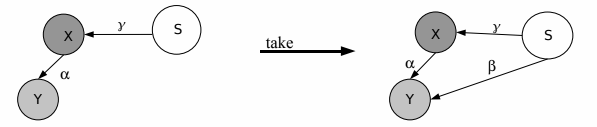
\includegraphics[width=0.7\textwidth]{./Pictures/takeRule.png}
	\caption[take rule]{\textit{Take} adds an edge from S to Y with the label $\beta \subseteq \alpha$. \cite{TakeG}}
	\label{fig:cltake}
\end{figure}	
	
\item \textbf{grant rule}:	Let S,X,Y agein be three distinct vertices in the graph with an arc, labelled with  $\alpha$, from S to Y and one labelled with $\gamma$ from S to X, such that g $\in \gamma$. "g" denotes the grant authority.
\begin{figure}[ht]
\centering
	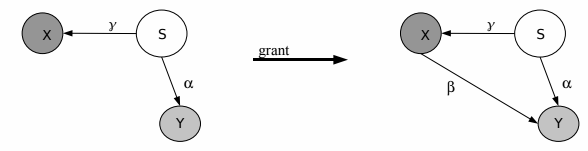
\includegraphics[width=0.7\textwidth]{./Pictures/grantRule.png}
	\caption[grant rule]{\textit{Grant} adds an edge from X to Y with the label $\beta \subseteq \alpha$.  \cite{TakeG}}
	\label{fig:clgrant}
\end{figure}	
	
\item \textbf{create rule}: Let S be a vertex in the graph. 
\begin{figure}[H]
\centering
	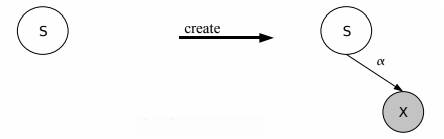
\includegraphics[width=0.5\textwidth]{./Pictures/createRule.png}
	\caption[create rule]{\textit{Create} adds a new node X and an arc from S to X, labelled with $\alpha$. \cite{TakeG}}
	\label{fig:clcreate}
\end{figure}	

\item \textbf{remove rule}: Let S, X be vertices in the graph with an arc from S to X, labelled with $\alpha$. 
\begin{figure}[H]
\centering
	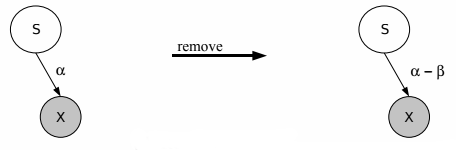
\includegraphics[width=0.5\textwidth]{./Pictures/removeRule.png}
	\caption[remove rule]{\textit{Remove} deletes $\beta$ labels from $\alpha$ or the arc itself if $\alpha - \beta = \lbrace\rbrace$. \cite{TakeG}}
	\label{fig:clremove}
\end{figure}		
\end{itemize}	
	
\subsubsection{Take-Grant specified for the seL4}\label{specT}
The Take-Grant Model specified in the paper "Verified Protection Model of the seL4 Microkernel" \cite{TakeG} is a variant of the classical Take-Grant model. In the paper the developers extended the original model in several ways. \\
From the modifications made the one on the \textit{create rule} is the most important one. As I explained in chapter \ref{sec:seL4} authority in the kernel is implemented with capabilities. Adding a new node to the protection graph in the model corresponds to the creation of a new object with a capability pointing on it in the kernel. Therefore the object executing the \texttt{create operation} needs a capability with \texttt{create} authority. \\
The \textit{remove rule} was modified as it does not remove parts of labels anymore but the whole capability. That means the complete arc pointing on an object is removed. \\
To diminish authority a capability has to be removed and newly created with diminished authority. \\
With \texttt{retype} newly created capabilities are saved in a \textit{Capability Derivation Tree} (CDT) as children of the UMO. A capability can be copied with the \texttt{mint} or \texttt{imitate operation}. \\ 
A capability  copied with \texttt{mint} is inserted in the CDT as child of the original one. Those that are copied with \texttt{imitate} are siblings. Figure \ref{fig:cdt} showes a CDT where C1 and C2 are created from the UMO via \texttt{retype}. C3 and C4 are copied from C1 via \texttt{mint}. So they have the same or less authority as C1. C1' is copied from C1 via \texttt{imitate}. This operation transfers the same rights to the new capability. As a consequence the capability is inserted a sibling of C1. \\
	\begin{figure}[H]
	\centering
	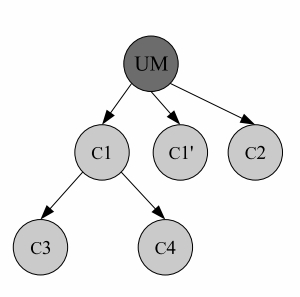
\includegraphics[width=0.3\textwidth]{./Pictures/CDT.jpg}
	\caption[CDT]{Example CDT with children and siblings \cite{PhDseL4}}
	\label{fig:cdt}
	\end{figure}
To remove a set of capabilities the operation \texttt{revoke} was implemented. \\ 
With this operation \texttt{remove} is executed on every capability that is in the CDT below the target capability. \\
The take rule was removed from the model and the grant rule was not modified: \\
An entity e$_1$, that has a capability with the grant right in it, pointing to an entity e$_2$ can give the same or less amount of rights on another entity to e$_2$. \\ 
A speciality of the extended model is, that objects and subjects are called \textit{entities}.\\
The goal of the paper "Verified Protection Model of the seL4 Microkernel" was to show that implementing isolated subsystems, using the mechanisms of the seL4 kernel, can be accomplished. \cite{TakeG} \\
Isolated subsystems are implemented as a collection of \textit{connected} entities. An entity that has \textit{grant authority} on another one is connected with this entity. Authority can neither get in nor get out of these isolated subsystems.\\
The exact specificaton of subsystems and entities follows in Chapter \ref{sec:Formalisation}.
\clearpage
% !TEX root = Bachelorarbeit.tex
\subsection{Noninterference}
Noninterference is an enhancement of the information flow model, first published by Goguen and Meseguer in 1982 and updated in 1984. It ensures that objects and subject from different security levels don't interfere with those at other levels. In the model variables are classified to be L (low security) or H (high security, private) variables. The goal is to prevent information to flow from H variables to L variables. \\
I use the noninterference formulation of Geoffrey Smith \cite{InfFlow}, which reads "Program c satisfies noninterference if, for any memories $\mu$ and $\nu$ that agree on L variables, the memories produced by running c on $\mu$ and on $\nu$ also agree on L variables (provided that both runs terminate successfully)." \\
This means that, if in a program two states are equivalent on a low level domain, then they are still equivalent on this level after a program was executed.\\
Central to to noninterference is the notion of a \textit{policy} $\leadsto$. It specifies the allowed information  flows between domain. $L \leadsto H$ if information is allowed to flow from domain L to domain H. \\
The model says two memories $\mu$ and $\nu$ agree on L variables if they fullfil an equivalence relation $\mu$ $\overset{\text{L}}{\sim}$ $\nu$. \\
The exact formalisation of noninterferenc for the validation follows in chapter \ref{FormNon}.
\newpage
% !TEX root = Bachelorarbeit.tex
\section{Formalisation of the Take-Grant Model}\label{sec:Formalisation}
\subsection{Capabilities}
In the Take-Grant model for seL4 \cite{TakeG}, where I got the formalisation from, the authors waived the usual differentation between subjects and objects and called all kernel objects \textit{entities}. \\ \\
The entities' memory address identifies them and is modeled as a natural number. \\ \\
	{\relsize{-1}
	\textbf{type$\_$synonym} \texttt{ entity$\_$id = nat}} \\ \\
With each capability a set of rights is associated. There are four access rights in the system model:	\\ \\
	{\relsize{-1}
	\textbf{datatype} \texttt{ rights = Read | Write | Grant | Create}} 
	
\begin{itemize}	
\item \textit{Read} authorises the reading of information from another entity. 
\item \textit{Write} authorises the writing of information to another entity. 
\item \textit{Grant} authorises the passing of a capability to another entity. 
\item \textit{Create} authorises the creation of new entities, which models the behavior of untyped memory objects. 
\end{itemize} 
	
A capability has two fields:
\begin{enumerate}
\item An identifier that names a target-entity
\item A set of rights that defines which system operations the source-entity is authorized to perform on the target-entity. 
\end{enumerate} 

	{\relsize{-1}
	\textbf{record} 
	\texttt{	
	\begin{tabular}[t]{ll}
	cap = & entity :: entity$\_$id \\
	      & rights :: rights set
	\end{tabular}} }
	\\ \\ \\
	
An entity has a set of capabilities: \\ \\
	{\relsize{-1}
	\textbf{record } \texttt{ 						
	entity = caps :: cap set}} \\ \\
	
The systems' state includes two fields: 
\begin{enumerate}
\item The \texttt{heap}, which stores the entities of the system like an array from address \texttt{0} up to and excluding \texttt{next$\_$id}.
\item \texttt{next$\_$id} contains slot for the next entity without overlapping with an existing one. 
\end{enumerate} 
	{\relsize{-1}	
	\textbf{record}
	\texttt{
	\begin{tabular}[t]{ll}
	state =	& heap :: entity$\_$id $\Rightarrow$ entity \\
			& next$\_$id :: entity$\_$id
	\end{tabular}}}  \\
	
\subsection{System Operations}\label{sec:System Operations}
The data type \texttt{sysOps} defines the different system operations of the seL4. \\ \\
	{\relsize{-1}	
	\textbf{datatype}
	\texttt{
	\begin{tabular}[t]{lll}
	sysOps	&	=	&	SysNoOp entity$\_$id \\
			&	|	&	SysRead	entity$\_$id cap \\
			&	|	&	SysWrite entity$\_$id cap \\
			&	|	&	SysCreate entity$\_$id cap cap \\
			&	|	&	SysGrant entity$\_$id cap cap rights set \\
			&	|	&	SysRemove	entity$\_$id cap cap \\
			&	|	&	SysRevoke entity$\_$id cap
	\end{tabular}}} \\ \\ 
	
The entity$\_$id in each operation is the entity initiating the operation. The first named capability is the one that is being invoked. The second capability for \texttt{SysCreate} points to the target entity for the new capability. For \texttt{SysGrant} it is the passed capability and for \texttt{SysRemove} it is the one that has to be removed. The rights set in \texttt{SysGrant} is necessary for the initiating entity to have the option only to transport a subset of the authority it offers to the receiver. 	\\

The \texttt{diminish} function applies this mask on the given acces rights: \\ \\
	{\relsize{-1}	
	\texttt{
	diminish :: "cap $\Rightarrow$ rights set $\Rightarrow$ cap" \textbf{where} \\
	diminish c R $\equiv$ c$\llparenthesis$rights := rights c $\cap$ \textit{R}$\rrparenthesis$}} \\ \\ \\
	
\texttt{legal} defines on what terms any system operation is allowed. \\ \\
	{\relsize{-1}
	\texttt{legal :: "sysOPs $\Rightarrow$ state $\Rightarrow$ bool" \texttt{where}}\\ \\
	
	\texttt{
	\begin{tabular}{lllll}
	  	&	"legal	&	(SysNoOp e) s	&	=	&	isEntityOf s e" \\
	|	& 	"legal	&	(SysCreate e c$_1$ c$_2$) s	&  =	& (isEntityOf s e $\wedge$ {c$_1$, c$_2$} $\subseteq$ caps$\_$of s e $\wedge$ \\ & & & & Grant $\in$ rights c$_2$ $\wedge$ Create $\in$ rights c$_2$)" \\
	| 	& "legal 	& 	(SysRead e c) s	&	=	&	(isEntityOf s e $\wedge$ c $\in$ caps$\_$of s e $\wedge$ Read \\ & & & & $\in$ rights c)" \\
	|	&	"legal 	&	(SysWrite e c) s&	= 	&	(isEntityOf s e $\wedge$ c $\in$ caps$\_$of s e $\wedge$ Write \\ & & & & $\in$ rights c)" \\
	| 	&	"legal 	&	(SysGrant e c$_1$ c$_2$ r) s & = & (isEntityOf s e $\wedge$  isEntityOf s (entity c$_1$) \\ & & & & $\wedge$ {c$_1$,c$_2$} $\subseteq$ caps$\_$of s e $\wedge$ Grant $\in$ rights c$_1$)" \\
	| 	&	"legal 	&	(SysRemove e c$_1$ c$_2$) s	&  =	& (isEntityOf s e $\wedge$ c$_1$ $\in$ caps$\_$of s e)" \\
	|	&	"legal	&	(SysRevoke e c) s	&	=	&	isEntityOf s e $\wedge$ c $\in$ caps$\_$of s e"
	\end{tabular}}} \\ \\ \\
	
The function \texttt{isEntityOf} tests the existence of an \texttt{entity$\_$id}. \texttt{Caps$\_$of} issues the set of all capabilities  contained in the entity with the address \texttt{r} in state \texttt{s}. \\ \\

	The \texttt{step'} and \texttt{step} functions define the execution of a single system operation. The original executions of \texttt{SysNoOp}, \texttt{SysRead} and \texttt{SysWrite} do not have an underlying function. All other functions are defined. \\ \\
	The \texttt{step} function: \\ \\
	{\relsize{-1}	
	\texttt{step' :: "sysOPs $\Rightarrow$ state $\Rightarrow$ state" \textbf{where}} \\
	\texttt{
	\begin{tabular}{lllll}
		&	"step'	&	(SysNoOp e) s	&	=	&	s" \\
	|	&	"step'	&	(SysRead e c) s	&	=	&	s" \\
	|	&	"step'	&	(SysWrite e c) s &	=	&	s" \\
	|	&	"step'	&	(SysCreat e c$_1$ c$_2$) s & = & createOperation e c$_1$ c$_2$ s" \\
	|	&	"step'	&	(SysGrant e c$_1$ c$_2$ \textit{R}) s & = & grantOperation e c$_1$ c$_2$ \textit{R} s" \\
	|	&	"step'	&	(SysRemove e c$_1$ c$_2$) s & = & removeOperation e c$_1$ c$_2$ s" \\
	|	&	"step'	&	(SysRevoke	e c) s & =	&	revokeOperation e c s" 
	\end{tabular}} \\ \\
	\texttt{step :: "sysOps $\Rightarrow$ state $\Rightarrow$ state" \textbf{where} \\
	step cmd s $\equiv$ if legal cmd s then step' cmd s else s}} \\ \\
	The defined functions for the system operations \texttt{create, grant, remove} and \texttt{revoke}: \\ \\
	{\relsize{-1}
	\texttt{createOperation :: "entity$\_$id $\Rightarrow$ cap $\Rightarrow$ cap $\Rightarrow$ modify$\_$state" \textbf{where}} \\
  \texttt{createOperation e c$_1$ c$_2$ s $\equiv$ \\
  \begin{tabular}{ll}
            let & nullEntity = $\llparenthesis$cap = {}, eValue = NULL$\rrparenthesis$ ; \\
                & newCap = $\llparenthesis$entity = next$\_$id s, rights = all$\_$rights$\rrparenthesis$; \\
                & newTarget = $\llparenthesis$caps = {newCap} ∪ caps$\_$of s (entity c$_2$), eValue = NULL$\rrparenthesis$ \\
             in & s$\llparenthesis$heap := (heap s)(entity c$_2$ := newTarget, next$\_$id s := nullEntity), next$\_$id := next$\_$id s+1$\rrparenthesis$"
   \end{tabular} \\ \\ \\
    grantOperation :: "entity$\_$id $\Rightarrow$ cap $\Rightarrow$ cap $\Rightarrow$ rights set $\Rightarrow$ modify$\_$state" \textbf{where} \\
  "grantOperation e c$_1$ c$_2$ \textit{R} s $\equiv$ \\
  s$\llparenthesis$heap := (heap s)(entity c$_1$ := $\llparenthesis$caps = {diminish c$_2$ \textit{R}} $\cup$ caps$\_$of s (entity c$_1$), eValue = value$\_$of s \\(entity c$_1$)$\rrparenthesis$)$\rrparenthesis$"\\ \\ \\
   removeOperation :: "entity$\_$id $\Rightarrow$ cap $\Rightarrow$ cap $\Rightarrow$ modify$\_$state" \textbf{where} \\
  "removeOperation c$_1$ c$_2$ s $\equiv$ s$\llparenthesis$heap := (heap s)(entity c$_1$ := $\llparenthesis$caps = caps$\_$of s (entity c$_1$) - {c$_2$}, eValue = value$\_$of s (entity c$_1$)$\rrparenthesis$)$\rrparenthesis$"}} 
\newpage
% !TEX root = Bachelorarbeit.tex
\section{Formalisation of the Noninterference Model}\label{FormNon}
For the validation a formalisation of the noninterference property. \\ 

{\relsize{-1}
\texttt{
noninterference :: "bool" \textbf{where} \\
"noninterference $\equiv$ $\forall$ \textit{a l h s t s' t'.}reachable \textit{s} $\wedge$ reachable \textit{t} $\wedge$ \textit{s $\overset{\text{l}}{\sim}$ t} $\wedge$ (\textit{h $\leadsto$ l $\longrightarrow$ \\
 s $\overset{\text{h}}{\sim}$ t}) $\wedge$ \textit{(s,s')}$\in$ Step \textit{a} $\wedge$ \textit{(t,t')}$\in$ Step \textit{a} $\longrightarrow$ \textit{s' $\overset{\text{l}}{\sim}$ t'}}"} \\ \\

"\texttt{a}" names the system operation, "\texttt{l}" a low level domain, "\texttt{h}" a high level domain, from the states "\texttt{s}" and "\texttt{t}" the system operation is executed and "\texttt{s'}" and "\texttt{t'}" are the resulting states. \\ \\
First I tried to validate confidentiality for the different system operations as they are defined in the take-grant-model. With this model it is impossible to decide whether a change of value has been recognized by another domain. \\
In the paper an entity only includes a set of capabilites. For my purpose I need the option to access the content of the entities, because the rules for noninterference state that no information is allowed to flow from one domain to another. This includes the information stored in the kernel objects. 
Therefore I extend the original record \texttt{entity} by adding a \textit{value} modelled by a natural number. \\ 

My entity type: \\ \\
	{\relsize{-1}
	\textbf{record} 
	\texttt{
	\begin{tabular}[t]{ll}
	entity = & caps :: cap set \\
			 & eValue :: nat 													
	\end{tabular}}} \\ \\ \\
	
To check noninterference I had to define a few functions. \\
	
\begin{enumerate}
	
\item The equivalence relation "$\sim$": \\
\texttt{s $\overset{\text{d}}{\sim}$ t} means that for every entity \texttt{e} reachable from an entity in \texttt{d} the status of \texttt{e} in \texttt{s} and \texttt{t} has to be the same. \\

I named the function \texttt{aquiv$\_$nonin}. It compares the value and capabilities of \texttt{e} and the entities of the subsystem \texttt{e} is located in for \texttt{s} and \texttt{t}. \\ \\
{\relsize{-1}
\texttt{
aquiv$\_$nonin :: "state $\Rightarrow$ state $\Rightarrow$ subSysT $\Rightarrow$ bool" \textbf{where} \\
"aquiv$\_$nonin s t d $\equiv$ $\{\forall$ e $\in$ d. value$\_$of s e = value$\_$of t e $\wedge$ caps$\_$of s e = \\
 caps$\_$of t e $\wedge$ subSys s e = subSys t e$\}$"}} \\

\item A function to read the value of an entity: \\ \\
{\relsize{-1}
\texttt{
value$\_$of :: "state $\Rightarrow$ entity$\_$id $\Rightarrow$ nat" where \\
"value$\_$of s sref $\equiv$ eValue(heap s sref)"}} \\

\item The isolation by using subsystems: \\
Subsystems are defined by entities that are \texttt{connected} with an entity \texttt{e} in a state \texttt{s}. \\ \\
To identify subsystems I need a datatype for them: \\ 

{\relsize{-1}\textbf{type$\_$synonym}
\texttt{
subSysT = "entity$\_$id st"}} \\ 

Now I can define Subsystems with the function \texttt{subSys}: \\ \\
{\relsize{-1}
\texttt{
subSys :: "state $\Rightarrow$ entity$\_$id $\Rightarrow$ subSysT" where \\ 
"subSys s e $\equiv$ $\{\forall$ e$_i$.in$\_$conc$\_$connected s e e$_i\}$"}} \\ \\
\texttt{in$\_$conc$\_$connected s e e$_i$} is true for entities \texttt{e} and \textbf{e$_i$} that are connected in state s. \\
\texttt{e} and \textbf{e$_i$} are connected in state \texttt{s} if a grant capability on \texttt{e$_i$} is part of \texttt{caps$\_$of e} or if a grant capability on \texttt{e} is part of \texttt{caps$\_$of e$_i$}.
\end{enumerate} 

The function \texttt{caps$\_$of e$_i$} was defined in chapter \ref{sec:Formalisation}. 
\newpage
% !TEX root = Bachelorarbeit.tex
\chapter{Validation of Noninterference}\label{ValNon}
After the formalisations in Chapter \ref{sec:Formalisation} and \ref{FormNon} I try to establish noninterference for the different system operations.\\ \\
First I tried to identify the conditions under which noninterference holds. For this I constructed a small model of the system with one Low-level-Subsystem and one High-level-Subsystem, with entities in them and tested for different right-sets and different operations if the noninterference-property holds. \\
The following displays this approach for the \texttt{write} operation from a low level domain on a high level domain. \\
I assume: \\ 
\begin{itemize}
\item H denotes a High level domain that implements the subsystem 'H'
\item L denotes a Low level domain that implements the subsystem 'L'
\item e$_1$ is an entity in H and e$_2$ is an entity in L
\item s $\overset{\text{L}}{\sim}$ t
\end{itemize} 
\begin{figure}[H]
\pgfuseimage{WriteGraphic1}
\caption{Noninterfernce of Write 1}
\end{figure}
To check noninterference I examine if the criterias for \texttt{aquiv$\_$nonin s' t' L} are fulfilled after the execution of the \texttt{write operation} and the named preconditions. \\ 
The \texttt{write operation} in the extended model satisfies the noninterference property: 
\begin{itemize}
\item We have \texttt{value$\_$of s' e = value$\_$of s e $\wedge$ caps$\_$of s' e = caps$\_$of s e} and \texttt{subSys s' e = subSys s e} as the \texttt{write operation} on the entity, \texttt{c$_1 \in e_2$} is pointing on, changes an entity e$_1 \in$ H and does not affect an entity $\in$ L.
\item We have \texttt{value$\_$of s e = value$\_$of t e $\wedge$ caps$\_$of s e = caps$\_$of t e} and \texttt{subSys s e = subSys t e} as one of the preconditions was s $\overset{\text{L}}{\sim}$ t. I defined the equivalence relation with the function aquiv$\_$nonin s t L, which is equal to the requirement. 
\item The \texttt{step} function first checks whether the execution of the system operation is legal, if not the new state t' equals the old state t. \\
\texttt{value$\_$of t e = value$\_$of t' e $\wedge$ caps$\_$of t e = caps$\_$of t' e} and \texttt{subSys t e = subSys t' e} as \texttt{write} is not part of c$_1$. So legal(SysWrite e$_2$ c$_1$) s = false what leads to t=t'. \\
\end{itemize} 
\textbf{In the following cases the proof looks always the same. So I shorten it:} \\ \\
\textbf{Preconditions:} \\ 
\begin{tabular}{ll}
* & s $\overset{\text{L}}{\sim}$ t $\Rightarrow$ aquiv$\_$nonin s t L	\\ 
** & writeOperation e$_2$ c$_1$  changes e$_1$ $\in$ H no e $\in$ L \\
*** & legal(SysWrite e$_2$ c$_1$) t = false $\Rightarrow$ t=t'
\end{tabular} \\ \\ 
\textbf{Proof of the noninterference property for Write 1:} \\ 
For all e$\in$L, we have: \\
\begin{tabular}{ll}
& (value$\_$of s' e $\overset{\text{**}}{=}$ value$\_$of s e $\overset{\text{*}}{=}$ value$\_$of t e $\overset{\text{***}}{=}$ value$\_$of t' e \\
$\wedge$ & caps$\_$of s' e $\overset{\text{**}}{=}$ caps$\_$of s e $\overset{\text{*}}{=}$ caps$\_$of t e $\overset{\text{***}}{=}$ caps$\_$of t' e \\
$\wedge$ & subSys s' e $\overset{\text{**}}{=}$ subSys s e $\overset{\text{*}}{=}$ subSys t e $\overset{\text{***}}{=}$ subSys t' e)
\end{tabular} \\
Hence aquiv$\_$nonin s' t' L , what is equivalent to s' $\overset{\text{L}}{\sim}$ t' \\ \\
\textbf{With s' $\overset{\text{L}}{\sim}$ t' the noninterference property for \texttt{write} is fulfilled.} 
\newpage
% !TEX root = Bachelorarbeit.tex
\section{Redesign of the take-grant-model}
This procedure worked until I came to the remove-operation. There I got the problem, that an entity in the given model is allowed to delete a capability and with that also an object in another domain without any restrictions:
\begin{figure}[H]
\pgfuseimage{RemoveGraphic1}
\caption{No confidentiality for Remove}
\end{figure}
In this example the L domain knows that the \texttt{removeOperation} was performed in the H domain as the capability c$_2$ was deleted. As a consequence the noninterference property is not achieved. \\
To study that problem I decided to classify the entities by their types, corresponding to the kernel specification \cite{Manual}:
\begin{itemize}
\item Untyped 
\item TCB
\item Synchronous IPC Endpoint (SEP)
\item Asychronous IPC Endpoint (AEP)
\item CNode
\item VSpace
\item Interrupt Controller 
\item Interrupt Handler
\item Shared Pages (Pages (Frames) can be shared between domains. The corresponding capability has to be copied and then mapped in the VSpace of the other domain.)
\end{itemize}
The following table shows the different object types with the different operation executable on them and the corresponding take- grant system calls: 
\begin{table}[H]
\begin{tabular}{|l|c|c|}
\hline
Capability Type & Concrete Kernel & protection model \\
\hline
\hline
Untyped & Retype & sequence of \textit{SysCreate} \\
& Revoke & \textit{SysRevoke} \\
\hline
TCB & TreadControl & \textit{SysNoOP, SysGrant} \\
& Exchange Registers & \textit{SystWrite} or \textit{SysRead} \\
& Yield & \textit{SysNoOP} \\
\hline
Synchronous IPC & Send IPC & \textit{SysWrite} or \textit{SysNoOP} \\
(Endpoint) & Wait IPC & \textit{SysRead} \\
& Grant IPC & \textit{SysWrite, SysGrant} or \textit{SysNoOP} \\
\hline
Asynchronous IPC & Send Event & \textit{SysWrite} \\
(AsyncEndpoint) & Wait Event & \textit{SysRead} \\
\hline
CNode & imitate & \textit{SysGrant} \\
& mint & \textit{SysGrant} \\
& Remove & \textit{SysRemove} \\
& Revoke & \textit{SysRevoke} \\
& Move & \textit{SysGrant, SysRemove} \\
& Recycle & \textit{SysRevoke}, sequence of \textit{SysRemove} \\
\hline
VSpace & Install Mapping & \textit{SysGrant} \\
& Remove Mapping & \textit{SysRemove} \\
& Remap & \textit{SysRemove, SysGrant} \\
& initialise & \textit{SysNoOP} \\
\hline
InterruptController & Register interrupt & \textit{SysGrant} \\
& Unregister interrupt &  \textit{SysRemove}\\
\hline
Interrupt Handler & Acknowledge interrupt & \textit{SysWrite}\\
\hline
\end{tabular}
\caption{Relationship: operation of concrete kernel $\longleftrightarrow$ of protection model \cite{PhDseL4}} \end{table}
To discem the different object types I need to revise the entity record and the preconditions for the different system operations. \\ \\ 
New dataype for the object types: \\
{\relsize{-1}
	\textbf{datatype} 
	\texttt{
	\begin{tabular}[t]{lll}
	eType & = & Untyped \\
			 & | & TCB \\
			 & | & SEP \\
			 & | & AEP \\
			 & | & SPage \\
			 & | & CNode \\
			 & | & VSpace \\
			 & | & IContr \\
			 & | & IHandl							
	\end{tabular}}} \\ \\
The final version of the \texttt{entity} record: \\
	{\relsize{-1}
	\textbf{record} 
	\texttt{
	\begin{tabular}[t]{ll}
	entity = & caps :: cap set \\
			 & eValue :: nat \\
			 & eType :: eType										
	\end{tabular}}} 
\clearpage
	The revised version of the \texttt{legal} function:\\
		{\relsize{-1}
	\texttt{legal :: "sysOPs $\Rightarrow$ state $\Rightarrow$ bool" \texttt{where}}\\ \\
	\texttt{
	\begin{tabular}{lllll}
	  	&	"legal	&	(SysNoOp e) s	&	=	&	isEntityOf s e" \\
	|	& 	"legal	&	(SysCreate e c$_1$ c$_2$) s	&  =	& (isEntityOf s e $\wedge$ {c$_1$, c$_2$} $\subseteq$ caps$\_$of s e $\wedge$ \\ & & & & Grant $\in$ rights c$_2$ $\wedge$ Create $\in$ rights c$_2$) $\wedge$ \\ & & & & eType (entity c$_1$ = Untyped" \\
	| 	& "legal 	& 	(SysRead e c) s	&	=	&	(isEntityOf s e $\wedge$ c $\in$ caps$\_$of s e $\wedge$ Read \\ & & & & $\in$ rights c) $\wedge$ eType (entity c) = TCB $\vee$ SEP $\vee$ AEP \\ $\vee$ SPage" \\
	|	&	"legal 	&	(SysWrite e c) s&	= 	&	(isEntityOf s e $\wedge$ c $\in$ caps$\_$of s e $\wedge$ Write \\ & & & & $\in$ rights c) $\wedge$ eType  (entity c) = TCB $\vee$ SEP $\vee$ AEP \\ & & & & $\vee$ IHandl $\vee$ SPage" \\
	| 	&	"legal 	&	(SysGrant e c$_1$ c$_2$ r) s & = & (isEntityOf s e $\wedge$  isEntityOf s (entity c$_1$) \\ & & & & $\wedge$ {c$_1$,c$_2$} $\subseteq$ caps$\_$of s e $\wedge$ Grant $\in$ rights c$_1$) $\wedge$ \\ & & & & eType (entity c$_1$)  = TCB $\vee$ SEP $\vee$ CNode $\vee$ VSpace $\vee$ \\ & & & & IContr" \\
	| 	&	"legal 	&	(SysRemove e c$_1$ c$_2$) s	&  =	& (isEntityOf s e $\wedge$ c$_1$ $\in$ caps$\_$of s e)  $\wedge$ \\ & & & & eType (entity c$_1$) = CNode $\vee$ VSpace $\vee$ IContr" \\
	|	&	"legal	&	(SysRevoke e c) s	&	=	&	isEntityOf s e $\wedge$ c $\in$ caps$\_$of s e  $\wedge$ \\ & & & & eType (entity c) = Untyped $\vee$ CNode"
	\end{tabular}}} \\ \\ \\
As mentioned in chapter \ref{sec:System Operations} (System Operations) the step function first proves whether a system operation is "legal" in state s. If it is, the system operation is performed. Otherwise the new state \texttt{s'} is defined as \texttt{s' = s}. This means that if a system operation is not legal nothing happens. 
For the validation I took a subsystem (SS1) of one Domain (D1) and another subsystem (SS2) of a second Domain (D2). \\
In chapter \ref{sec:KernelObjects} (Kernel Objects) I explained that the only communication between Domains goes through \textit{Asynchronous Endpoints} and \textit{Shared Pages}. \\
Figure \ref{overview} pictures an example of how the objects and methods can be placed in the domains and how the connection to \textit{Asynchronous Endpoints} and \textit{Shared Pages} is implemented if the information is allowed to flow from Domain 1 to Domain 2: D1$\leadsto$D2 but D2$\not\leadsto$D1.
\begin{flushleft}
\begin{figure}[H]
\pgfuseimage{OverviewObjects}
\caption{Objects and Methods in the kernel}
\label{overview}
\end{figure}
\end{flushleft}
\newpage
\section{Validation with the new model}\label{sec:ValNew}
I examine each operation of the protection model and distinguish therefore between the different object types. \\
For this I assume that Domain 1 equates a low level domain and Domain 2 a high level domain. So  information is allowed to flow from Domain 1 to Domain 2 but not from Domain 2 to Domain 1. \\ \\
\textbf{D1$\leadsto$D2 but D2$\not\leadsto$D1} \\ \\
Further I assume that state s is equivalent to state t for Domain 1. What is represented by the function  \texttt{aquiv$\_$nonin} \\ \\
\textbf{s $\overset{\text{D1}}{\sim}$ t $\equiv$ aquiv$\_$nonin s t D1}	\\ \\
In this chapter I show that the criteria for the equivalence relation still holds in Domain 1, between s' and t', after every type of operation. 
% !TEX root = Bachelorarbeit.tex
\section{Create}\label{sec:Create}
Create corresponds to the \textit{Retype} operation on untyped memory objects (UMOs). Each Domain has a own and fixed section of memory. So the UMO for the \texttt{retype} is located in the same Domain as the implementing entity. Furthermore the created entity is placed in the same Domain as in the CDT it is a child of the UMO.  
\subsection{Create on UMO}
The following picture shows how a create operation in a \texttt{H} domain changes or not the equivalence criteria in the \texttt{L} domain that is not allowed to get information from the former one. \\
Each domain includes a subsystem. D1 includes the subsystem SS1 and D2 the subsystem SS2. Each figure has four subfigures. The first one in the left upper corner showes the state s before the execution of the \texttt{create} operation. The one on the right of it shows state s' after the execution of the \texttt{create} operation with the changed subsystems. \\
The subfigure on left lower corner showes the state t before the execution of the \texttt{create} operation. The one on the right of it shows state t' after the execution of the \texttt{create} operation with the changed subsystems.
\begin{figure}[H]
\pgfuseimage{CreateUMO}
\caption{Noninterference for Create on Untyped Memory Objects}
\end{figure}
I have to show that if s $\overset{\text{D1}}{\sim}$ t and (s,s') $\in$ Step a and (t,t') $\in$ Step a then s' $\overset{\text{D1}}{\sim}$ t'. 
s $\overset{\text{D1}}{\sim}$ t was defined in Chapter \ref{ValNew} as the boolean fuction aquiv$\_$nonin s t D1. The function is true if all entities e $\in$ D1 have the same value in s and t (value$\_$of s e = value$\_$of t e), if they also have the same capabilities in s and t (caps$\_$of s e = caps$\_$of t e) and if D1 has the same entities in s and t (subSys s e = subSys t e).\\
In the following Section I check if value$\_$of s' e = value$\_$of t' e, caps$\_$of s' e = caps$\_$of t’ e and subSys s' e = subSys t' e for all e $\in$ D1 after the execution of 
createOperation e$_2$ c$_1$ c$_2$ s respectively createOperation e$_2$ c$_1$ c$_2$ t. If that is the case I can say that aquiv$\_$nonin s' t' D1 = true. From my definition of \texttt{aquiv$\_$nonin} this leads to s' $\overset{\text{D1}}{\sim}$ t'. \\ 
\textbf{Preconditions:} \\ \\
\begin{tabular}{ll}
* & s $\overset{\text{D1}}{\sim}$ t $\equiv$ \texttt{aquiv$\_$nonin s t D1}	\\ 
** & createOperation e$_2$ c$_1$ c$_2$ s creates e$_3$ $\in$ D2 and doesn't change or create any e $\in$ \\
&  D1 \\
*** & legal (SysCreate e$_2$ c$_1$ c$_2$) t = false $\Rightarrow$ t' = t
\end{tabular}\\ \\ 
\textbf{Proof of the noninterference property for create on UMO:} \\ \\
For all e $\in$ D1, we have: \\ 
\begin{tabular}{ll}
& (value$\_$of s' e $\overset{\text{**}}{=}$ value$\_$of s e $\overset{\text{*}}{=}$ value$\_$of t e $\overset{\text{***}}{=}$ value$\_$of t' e \\
$\wedge$ & caps$\_$of s' e $\overset{\text{**}}{=}$ caps$\_$of s e $\overset{\text{*}}{=}$ caps$\_$of t e $\overset{\text{***}}{=}$ caps$\_$of t' e \\
$\wedge$ & subSys s' e $\overset{\text{**}}{=}$ subSys s e $\overset{\text{*}}{=}$ subSys t e $\overset{\text{***}}{=}$ subSys t' e)
\end{tabular} \\
Hence aquiv$\_$nonin s' t' D1 , what is equivalent to s' $\overset{\text{D1}}{\sim}$ t' \\ \\ 
\textbf{With s' $\overset{\text{D1}}{\sim}$ t' the noninterference property for \texttt{create} on an untyped memory object is fulfilled.} 
\subsection{Create on all other object types inside a domain}
If \texttt{create} is performed on another object type than an untyped memory object, the  function step' (SysCreate e c$_1$ c$_2$)s does nothing. So the new state \texttt{s'} equates the old state \texttt{s}. \\
The following figure shows the createOperation for every other object type inside a domain.\\
\begin{figure}[H]
\pgfuseimage{CreateOther}
\caption{Noninterference for Create on object types $\neq$ Untyped Memory Objects}
\end{figure} 
\textbf{Preconditions:} \\ \\
\begin{tabular}{ll}
* & s $\overset{\text{D1}}{\sim}$ t $\equiv$ \texttt{aquiv$\_$nonin s t D1}	\\ 
** & legal (SysCreate e$_2$ c$_1$ c$_2$) s = false $\Rightarrow$ s' = s \\ 
*** & legal (SysCreate e$_2$ c$_1$ c$_2$) t = false $\Rightarrow$ t' = t
\end{tabular}\\ \\  
\textbf{Proof of the noninterference property for create on other object types in a domain:} \\ \\
For all e $\in$ D1, we have: \\ 
\begin{tabular}{ll}
& (value$\_$of s' e $\overset{\text{**}}{=}$ value$\_$of s e $\overset{\text{*}}{=}$ value$\_$of t e $\overset{\text{***}}{=}$ value$\_$of t' e \\
$\wedge$ & caps$\_$of s' e $\overset{\text{**}}{=}$ caps$\_$of s e $\overset{\text{*}}{=}$ caps$\_$of t e $\overset{\text{***}}{=}$ caps$\_$of t' e \\
$\wedge$ & subSys s' e $\overset{\text{**}}{=}$ subSys s e $\overset{\text{*}}{=}$ subSys t e $\overset{\text{***}}{=}$ subSys t' e)
\end{tabular} \\
Hence aquiv$\_$nonin s' t' D1 , what is equivalent to s' $\overset{\text{D1}}{\sim}$ t' \\ \\ 
\textbf{With s' $\overset{\text{D1}}{\sim}$ t' the noninterference property for \texttt{create} on other object types in a domain is fulfilled.} 
\subsection{Create on Asynchronous IPC Endpoint or Shared Page objects}
Next I want to be sure that create has no impact on the entities in the L domain if it is executed on AEP or SPage objects.\\
\begin{figure}[H]
\pgfuseimage{CreateOutside}
\caption{Noninterference for Create on object types = AEP $\vee$ SPage}
\end{figure}
In this case the check if the execution is legal = false in both states. So in both states the step' function leads to the definition of the old state. \\ \\
\textbf{Preconditions:} \\ \\
\begin{tabular}{ll}
* & s $\overset{\text{D1}}{\sim}$ t $\equiv$ \texttt{aquiv$\_$nonin s t D1}	\\ 
** & legal (SysCreate e$_2$ c$_1$ c$_2$) s = false $\Rightarrow$ s' = s \\ 
*** & legal (SysCreate e$_2$ c$_1$ c$_2$) t = false $\Rightarrow$ t' = t
\end{tabular}\\ \\ 
\textbf{Proof of the noninterference property for \texttt{create} on Asynchronous IPC Endpoint or Shared Page objects:}\\ \\
For all e $\in$ D1, we have: \\ 
\begin{tabular}{ll}
& (value$\_$of s' e $\overset{\text{**}}{=}$ value$\_$of s e $\overset{\text{*}}{=}$ value$\_$of t e $\overset{\text{***}}{=}$ value$\_$of t' e \\
$\wedge$ & caps$\_$of s' e $\overset{\text{**}}{=}$ caps$\_$of s e $\overset{\text{*}}{=}$ caps$\_$of t e $\overset{\text{***}}{=}$ caps$\_$of t' e \\
$\wedge$ & subSys s' e $\overset{\text{**}}{=}$ subSys s e $\overset{\text{*}}{=}$ subSys t e $\overset{\text{***}}{=}$ subSys t' e)
\end{tabular} \\
Hence aquiv$\_$nonin s' t' D1 , what is equivalent to s' $\overset{\text{D1}}{\sim}$ t' \\ \\ 
\textbf{With s' $\overset{\text{D1}}{\sim}$ t' the noninterference property for \texttt{create} on Asynchronous IPC Endpoint or Shared Page objects is fulfilled.} 
\clearpage
% !TEX root = Bachelorarbeit.tex
\section{Grant}\label{sec:Grant}
The \texttt{grant} operation can only be performed inside a domain on a TCB, Synchronous IPC, CNode, VSpace or Interrupt Controller object. 
\subsection{Grant on TCB, SEP, CNode, VSpace or IContr objects} 
Now I show that any \texttt{grant} operation inside a H domain on one of the named objects does not affect the values, capabilities or entities of an L domain. \\
As every given object behaves in the same way, I generalized e$_4$ = TCB $\vee$ SEP $\vee$ CNode $\vee$ VSpace $\vee$ IContr.
\begin{figure}[H]
\pgfuseimage{GrantTCB}
\caption{Noninterference for Grant on an TCB, Synchronous IPC Endpoint, CNode, VSpace or Interrupt Controller object.}
\end{figure}
The \texttt{grant} operation has no impact on the entities of the other domain because it adds a capability to an entity inside the domain, which also contains the target and source entities. \\ \\
\textbf{Preconditions:} \\ \\
\begin{tabular}{ll}
* & s $\overset{\text{D1}}{\sim}$ t $\equiv$ aquiv$\_$nonin s t D1	\\ 
** & grantOperation e$_2$ c$_1$ c$_2$ R s creates c$_3$ $\in$ D2 and does not change or create any \\
& capability $\in$ D1 \\ 
*** & legal (SysGrant e$_2$ c$_1$ c$_2$ R) t = false $\Rightarrow$ t' = t
\end{tabular}\\ \\ 
\textbf{Proof of the noninterference property for \texttt{grant} on TCB, Synchronous IPC Endpoint, CNode, VSpace and Interrupt Controller objects:}\\ \\
For all e $\in$ D1, we have: \\ 
\begin{tabular}{ll}
& (value$\_$of s' e $\overset{\text{**}}{=}$ value$\_$of s e $\overset{\text{*}}{=}$ value$\_$of t e $\overset{\text{***}}{=}$ value$\_$of t' e \\
$\wedge$ & caps$\_$of s' e $\overset{\text{**}}{=}$ caps$\_$of s e $\overset{\text{*}}{=}$ caps$\_$of t e $\overset{\text{***}}{=}$ caps$\_$of t' e \\
$\wedge$ & subSys s' e $\overset{\text{**}}{=}$ subSys s e $\overset{\text{*}}{=}$ subSys t e $\overset{\text{***}}{=}$ subSys t' e)
\end{tabular} \\
Hence aquiv$\_$nonin s' t' D1, what is equivalent to s' $\overset{\text{D1}}{\sim}$ t'. \\ \\ 
\textbf{With s' $\overset{\text{D1}}{\sim}$ t' the noninterference property for \texttt{grant} on TCB, Synchronous IPC Endpoint, CNode, VSpace and Interrupt Controller objects is fulfilled.} 
\subsection{Grant on other objects inside a domain} 
In this paragraph I will check if an execution of the \texttt{grant} operation on another object than TCB, SEP, CNode, VSpace, Interrupt Controller or the object types that establish a communication interface between domains: AEP and SPage, alters the configuration of the other domain. \\ \\
\begin{figure}[H]
\pgfuseimage{GrantOthers}
\caption{Noninterference for Grant on an object $\neq$ TCB, SEP, CNode, VSpace, IContr, SPage or AEP object.}
\end{figure}
\textbf{Preconditions:} \\ \\
\begin{tabular}{ll}
* & s $\overset{\text{D1}}{\sim}$ t $\equiv$ aquiv$\_$nonin s t D1	\\ 
** & legal (SysGrant e$_2$ c$_1$ c$_2$) s = false $\Rightarrow$ s' = s \\ 
*** & legal (SysGrant e$_2$ c$_1$ c$_2$ R) t = false $\Rightarrow$ t' = t
\end{tabular}\\ \\ 
\textbf{Proof of the noninterference property for \texttt{grant} on an object $\neq$ TCB, SEP, CNode, VSpace, IContr, SPage or AEP:}\\ \\
For all e $\in$ D1, we have: \\ 
\begin{tabular}{ll}
& (value$\_$of s' e $\overset{\text{**}}{=}$ value$\_$of s e $\overset{\text{*}}{=}$ value$\_$of t e $\overset{\text{***}}{=}$ value$\_$of t' e \\
$\wedge$ & caps$\_$of s' e $\overset{\text{**}}{=}$ caps$\_$of s e $\overset{\text{*}}{=}$ caps$\_$of t e $\overset{\text{***}}{=}$ caps$\_$of t' e \\
$\wedge$ & subSys s' e $\overset{\text{**}}{=}$ subSys s e $\overset{\text{*}}{=}$ subSys t e $\overset{\text{***}}{=}$ subSys t' e)
\end{tabular} \\
Hence aquiv$\_$nonin s' t' D1, what is equivalent to s' $\overset{\text{D1}}{\sim}$ t'. \\ \\ 
\textbf{With s' $\overset{\text{D1}}{\sim}$ t' the noninterference property for \texttt{grant} on an object $\neq$ TCB, SEP, CNode, VSpace, IContr, SPage or AEP is fulfilled.} 
\subsection{Grant on Asynchronous IPC Endpoint or Shared Page objects}
The next figure illustrates \texttt{grant} on the two object types connecting different domains. In both cases the operation is not legal. So the new state equates the old one.
\begin{figure}[H]
\pgfuseimage{GrantOutside}
\caption{Noninterference for Grant on an Asychronous IPC Endpoint object.}
\end{figure}
\textbf{Preconditions:} \\ \\
\begin{tabular}{ll}
* & s $\overset{\text{D1}}{\sim}$ t $\equiv$ aquiv$\_$nonin s t D1	\\ 
** & legal (SysGrant e$_2$ c$_1$ c$_2$) s = false $\Rightarrow$ s' = s \\ 
*** & legal (SysGrant e$_2$ c$_1$ c$_2$) t = false $\Rightarrow$ t' = t
\end{tabular}\\ \\ 
\textbf{Proof of the noninterference property for \texttt{grant} on an object = SPage or AEP:}\\ \\
For all e $\in$ D1, we have: \\ 
\begin{tabular}{ll}
& (value$\_$of s' e $\overset{\text{**}}{=}$ value$\_$of s e $\overset{\text{*}}{=}$ value$\_$of t e $\overset{\text{***}}{=}$ value$\_$of t' e \\
$\wedge$ & caps$\_$of s' e $\overset{\text{**}}{=}$ caps$\_$of s e $\overset{\text{*}}{=}$ caps$\_$of t e $\overset{\text{***}}{=}$ caps$\_$of t' e \\
$\wedge$ & subSys s' e $\overset{\text{**}}{=}$ subSys s e $\overset{\text{*}}{=}$ subSys t e $\overset{\text{***}}{=}$ subSys t' e)
\end{tabular} \\
Hence aquiv$\_$nonin s' t' D1, what is equivalent to s' $\overset{\text{D1}}{\sim}$ t'. \\ 
\textbf{With s' $\overset{\text{D1}}{\sim}$ t' the noninterference property for \texttt{grant} on an object = SPage or AEP is fulfilled.} 
\clearpage
% !TEX root = Bachelorarbeit.tex
\section{Write}\label{Write}
\texttt{Write} can be executed on TCB, SEP, AEP, SPage and Interrupt Handler objects.
\subsection{Write on TCB, SEP or IHandl objects}
I start with the \texttt{write} operation on all executable objects inside a domain. So in the next figure e$_3$ = TCB $\vee$ SEP $\vee$ IHandl.
\begin{figure}[H]
\pgfuseimage{WriteTCB}
\caption{Noninterference for Write on a TCB, Sychronous IPC Endpoint or Interrupt Handler object}
\end{figure}
\textbf{Preconditions:} \\ \\
\begin{tabular}{ll}
* & s $\overset{\text{D1}}{\sim}$ t $\equiv$ aquiv$\_$nonin s t D1	\\ 
** & writeOperation e$_2$ c$_1$ s only changes the value of an entity $\in$ D2 nothing in D1 \\ 
*** & legal (SysWrite e$_2$ c$_1$) t = false $\Rightarrow$ t' = t
\end{tabular} \\ \\ 
\textbf{Proof of the noninterference property for \texttt{write} on TCB, SEP or IHandl objects:}\\ \\
For all e $\in$ D1, we have: \\ 
\begin{tabular}{ll}
& (value$\_$of s' e $\overset{\text{**}}{=}$ value$\_$of s e $\overset{\text{*}}{=}$ value$\_$of t e $\overset{\text{***}}{=}$ value$\_$of t' e \\
$\wedge$ & caps$\_$of s' e $\overset{\text{**}}{=}$ caps$\_$of s e $\overset{\text{*}}{=}$ caps$\_$of t e $\overset{\text{***}}{=}$ caps$\_$of t' e \\
$\wedge$ & subSys s' e $\overset{\text{**}}{=}$ subSys s e $\overset{\text{*}}{=}$ subSys t e $\overset{\text{***}}{=}$ subSys t' e)
\end{tabular} \\
Hence aquiv$\_$nonin s' t' D1 , what is equivalent to s' $\overset{\text{D1}}{\sim}$ t' \\ \\ 
\textbf{With s' $\overset{\text{D1}}{\sim}$ t' the noninterference property for \texttt{write} on TCB, SEP or IHandl objects is fulfilled.} 
\subsection{Write on objects $\neq$ TCB, SEP, IHandl, SPage and AEP}\label{WriteOthers}
Like in \ref{sec:Create} Create and \ref{sec:Grant} Grant there are other object types inside a domain, which are not executeable with the \texttt{write} operation. Those are CNodes, VSpaces, UMOs and Interrupt Controllers. \\
\texttt{Write} operation on these objects: \\
\begin{figure}[H]
\pgfuseimage{WriteOthers}
\caption{Noninterference for Write on objects $\neq$ TCB, SEP, IHandl, SPage and AEP}
\end{figure}
\textbf{Preconditions:} \\ \\
\begin{tabular}{ll}
* & s $\overset{\text{D1}}{\sim}$ t $\equiv$ aquiv$\_$nonin s t D1	\\ 
** & legal (SysWrite e$_2$ c$_1$) s = false $\Rightarrow$ s' = s \\ 
*** & legal (SysWrite e$_2$ c$_1$) t = false $\Rightarrow$ t' = t
\end{tabular} \\ \\ 
\textbf{Proof of the noninterference property for \texttt{write} on objects $\neq$ TCB, SEP, IHandl, SPage and AEP:}\\ \\
For all e $\in$ D1, we have: \\ 
\begin{tabular}{ll}
& (value$\_$of s' e $\overset{\text{**}}{=}$ value$\_$of s e $\overset{\text{*}}{=}$ value$\_$of t e $\overset{\text{***}}{=}$ value$\_$of t' e \\
$\wedge$ & caps$\_$of s' e $\overset{\text{**}}{=}$ caps$\_$of s e $\overset{\text{*}}{=}$ caps$\_$of t e $\overset{\text{***}}{=}$ caps$\_$of t' e \\
$\wedge$ & subSys s' e $\overset{\text{**}}{=}$ subSys s e $\overset{\text{*}}{=}$ subSys t e $\overset{\text{***}}{=}$ subSys t' e)
\end{tabular} \\
Hence aquiv$\_$nonin s' t' D1 , what is equivalent to s' $\overset{\text{D1}}{\sim}$ t'\\ \\ 
\textbf{With s' $\overset{\text{D1}}{\sim}$ t' the noninterference property for \texttt{write} on objects $\neq$ TCB, SEP, IHandl, SPage and AEP is fulfilled.} 
\subsection{Write on AEP or SPage objects from Domain 2}\label{WriteOut}
In Chapter \ref{sec:ValNew} I defined the precondition $\Rightarrow$ D1$\leadsto$D2 but D2$\not\leadsto$D1. That means the rights from Domain 2 on Asychronous Endpoints and Shared Pages are restricted to \texttt{read}. 
If the write operation is called from Domain 2 it looks like it is illustrated in Figure \ref{fig:WriteOut1}. The policy prescribes that information is only allowed to flow from Domain 1 to Domain 2 but not from Domain 2 to Domain 1. As a consequence \texttt{write} can not be part of c$_1$. 
\begin{figure}[H]
\pgfuseimage{WriteOutside}
\caption{Noninterference for Write on an object = AEP executed from an entity $\in$ Domain 2}
\label{fig:WriteOut1}
\end{figure}
\textbf{Preconditions:} \\ \\
\begin{tabular}{ll}
* & s $\overset{\text{D1}}{\sim}$ t $\equiv$ aquiv$\_$nonin s t D1	\\ 
** & legal (SysWrite e$_2$ c$_1$) s = false $\Rightarrow$ s' = s \\ 
*** & legal (SysWrite e$_2$ c$_1$) t = false $\Rightarrow$ t' = t
\end{tabular} \\ \\ 
\textbf{Proof of the noninterference property for \texttt{write} on AEP or SPage objects from Domain 2:}\\ \\
For all e $\in$ D1, we have: \\ 
\begin{tabular}{ll}
& (value$\_$of s' e $\overset{\text{**}}{=}$ value$\_$of s e $\overset{\text{*}}{=}$ value$\_$of t e $\overset{\text{***}}{=}$ value$\_$of t' e \\
$\wedge$ & caps$\_$of s' e $\overset{\text{**}}{=}$ caps$\_$of s e $\overset{\text{*}}{=}$ caps$\_$of t e $\overset{\text{***}}{=}$ caps$\_$of t' e \\
$\wedge$ & subSys s' e $\overset{\text{**}}{=}$ subSys s e $\overset{\text{*}}{=}$ subSys t e $\overset{\text{***}}{=}$ subSys t' e)
\end{tabular} \\
Hence aquiv$\_$nonin s' t' D1 , what is equivalent to s' $\overset{\text{D1}}{\sim}$ t'\\ \\ 
\textbf{With s' $\overset{\text{D1}}{\sim}$ t' the noninterference property for \texttt{write} on AEP or SPage objects from Domain 2 is fulfilled.}  
\clearpage
\subsection{Write on an AEP or SPage object from Domain 1}\label{WriteOut2}
Write on AEP objects can be executed from Domain 1. Figure \ref{fig:WriteOut2} shows that this has no influence on the noninterference property.
\begin{figure}[H]
\pgfuseimage{WriteOutside2}
\caption{Noninterference for Write on an object = AEP executed from an entity $\in$ D1}
\label{fig:WriteOut2}
\end{figure}
\textbf{Preconditions:} \\ \\
\begin{tabular}{ll}
* & s $\overset{\text{D1}}{\sim}$ t $\equiv$ aquiv$\_$nonin s t D1	\\ 
** & writeOperation e$_1$ c$_1$ s changes the value $\in$ e$_3$ $\notin$ D1. \\
& That means it has no impact on any entity $\in$ D1 \\ 
*** & legal (SysWrite e$_2$ c$_1$) t = false $\Rightarrow$ t' = t
\end{tabular} \\ \\ 
\textbf{Proof of the noninterference property for \texttt{write} on AEP or SPage objects from Domain 1:}\\ \\
For all e $\in$ D1, we have: \\ 
\begin{tabular}{ll}
& (value$\_$of s' e $\overset{\text{**}}{=}$ value$\_$of s e $\overset{\text{*}}{=}$ value$\_$of t e $\overset{\text{***}}{=}$ value$\_$of t' e \\
$\wedge$ & caps$\_$of s' e $\overset{\text{**}}{=}$ caps$\_$of s e $\overset{\text{*}}{=}$ caps$\_$of t e $\overset{\text{***}}{=}$ caps$\_$of t' e \\
$\wedge$ & subSys s' e $\overset{\text{**}}{=}$ subSys s e $\overset{\text{*}}{=}$ subSys t e $\overset{\text{***}}{=}$ subSys t' e)
\end{tabular} \\
Hence aquiv$\_$nonin s' t' D1 , what is equivalent to s' $\overset{\text{D1}}{\sim}$ t'\\ \\ 
\textbf{With s' $\overset{\text{D1}}{\sim}$ t' the noninterference property for \texttt{write} on AEP or SPage objects from Domain 1 is fulfilled.}  
\clearpage
% !TEX root = Bachelorarbeit.tex
\subsection{Read}\label{sec:Read}
Read is legal on TCB, Sychronous IPC Endpoint, Asynchronous IPC Endpoint and Shared Page objects. \\
Like in chapter \ref{Write} I distinguish between objects with legal execution of \texttt{read} on objects inside a domain, illegal execution of \texttt{read} on objects inside a domain and both on objects outside a domain.
\subsubsection{Read on TCB or Sychronous IPC Endpoint objects}
TCB and SEP objects are the two object types that are executable with \texttt{read} from an endpoint in the same domain. \\
Figure \ref{fig:ReadTCB} illustrates whether the operation influences the L domain.
\begin{flushleft}
\begin{figure}[H]
\pgfuseimage{ReadTCB}
\caption{Noninterference for Read on a TCB or Sychronous IPC Endpoint object}
\label{fig:ReadTCB}
\end{figure}
\end{flushleft}
\textbf{Preconditions:} \\ \\
\begin{tabular}{ll}
* & s $\overset{\text{D1}}{\sim}$ t $\equiv$ aquiv$\_$nonin s t D1	\\ 
** & readOperation e$_2$ c$_1$ s only changes the value of an entity $\in$ D2 nothing in D1 \\ 
*** & legal (SysRead e$_2$ c$_1$) t = false $\Rightarrow$ t' = t
\end{tabular} \\ \\ 
\textbf{Proof of the noninterference property for \texttt{read} on TCB or SEP objects:}\\ \\
$\forall$ e $\in$ D1. \\ 
\begin{tabular}{ll}
& (value$\_$of s' e $\overset{\text{**}}{=}$ value$\_$of s e $\overset{\text{*}}{=}$ value$\_$of t e $\overset{\text{***}}{=}$ value$\_$of t' e \\
$\wedge$ & caps$\_$of s' e $\overset{\text{**}}{=}$ caps$\_$of s e $\overset{\text{*}}{=}$ caps$\_$of t e $\overset{\text{***}}{=}$ caps$\_$of t' e \\
$\wedge$ & subSys s' e $\overset{\text{**}}{=}$ subSys s e $\overset{\text{*}}{=}$ subSys t e $\overset{\text{***}}{=}$ subSys t' e)
\end{tabular} \\
$\Rightarrow$ aquiv$\_$nonin s' t' D1 $\Rightarrow$ s' $\overset{\text{D1}}{\sim}$ t' \\ \\
\textbf{With s' $\overset{\text{D1}}{\sim}$ t' the noninterference property for \texttt{read} on TCB or SEP objects is fulfilled.}  
\clearpage
\subsubsection{Read on other object types inside a domain} 
Figure \ref{fig:ReadOthers} depicts the read operation on objects in the same domain on which \texttt{read} is not executable. It is similar to \texttt{write} in chapter \ref{WriteOthers}.
\begin{flushleft}
\begin{figure}[H]
\pgfuseimage{ReadOthers}
\caption{Noninterference for Read on objects $\neq$ TCB, Asynchronous IPC Endpoint, Sychronous IPC Endpoint or Shared Page}
\label{fig:ReadOthers}
\end{figure}
\end{flushleft}
\textbf{Preconditions:} \\ \\
\begin{tabular}{ll}
* & s $\overset{\text{D1}}{\sim}$ t $\equiv$ aquiv$\_$nonin s t D1	\\ 
** & legal (SysRead e$_2$ c$_1$) s = false $\Rightarrow$ s' = s \\ 
*** & legal (SysRead e$_2$ c$_1$) t = false $\Rightarrow$ t' = t
\end{tabular} \\ \\ \\
\textbf{Proof of the noninterference property for \texttt{read} on objects $\neq$ TCB, SEP, SPage and AEP:}\\ \\
$\forall$ e $\in$ D1. \\ 
\begin{tabular}{ll}
& (value$\_$of s' e $\overset{\text{**}}{=}$ value$\_$of s e $\overset{\text{*}}{=}$ value$\_$of t e $\overset{\text{***}}{=}$ value$\_$of t' e \\
$\wedge$ & caps$\_$of s' e $\overset{\text{**}}{=}$ caps$\_$of s e $\overset{\text{*}}{=}$ caps$\_$of t e $\overset{\text{***}}{=}$ caps$\_$of t' e \\
$\wedge$ & subSys s' e $\overset{\text{**}}{=}$ subSys s e $\overset{\text{*}}{=}$ subSys t e $\overset{\text{***}}{=}$ subSys t' e)
\end{tabular} \\
$\Rightarrow$ aquiv$\_$nonin s' t' D1 $\Rightarrow$ s' $\overset{\text{D1}}{\sim}$ t' \\ \\ \\
\textbf{With s' $\overset{\text{D1}}{\sim}$ t' the noninterference property for \texttt{read} on objects $\neq$ TCB, SEP, SPage and AEP is fulfilled.}  
\clearpage
\subsubsection{Read on AEP or SPage objects from Domain 1}
Similar to chapter \ref{WriteOut} \texttt{read} can only be executed from a \texttt{H} domain. That is the one to which information is allowed to flow. In my case it is domain 2. No information is allowed to flow to domain 1. So \texttt{read} is not legal if it is executed from domain 1.\\
Figure \ref{fig:ReadOut} shows that this does not affect domain 1. 
\begin{flushleft}
\begin{figure}[H]
\pgfuseimage{ReadOutside2}
\caption{Noninterference for Read on object types = Asynchronous IPC Endpoint executed from Domain 1}
\label{fig:ReadOut}
\end{figure}
\end{flushleft} 
\textbf{Preconditions:} \\ \\
\begin{tabular}{ll}
* & s $\overset{\text{D1}}{\sim}$ t $\equiv$ aquiv$\_$nonin s t D1	\\ 
** & legal (SysRead e$_1$ c$_1$) s = false $\Rightarrow$ s' = s \\ 
*** & legal (SysRead e$_1$ c$_1$) t = false $\Rightarrow$ t' = t
\end{tabular} \\ \\ \\
\textbf{Proof of the noninterference property for \texttt{read} on AEP or SPage objects from Domain 1:}\\ \\
$\forall$ e $\in$ D1. \\ 
\begin{tabular}{ll}
& (value$\_$of s' e $\overset{\text{**}}{=}$ value$\_$of s e $\overset{\text{*}}{=}$ value$\_$of t e $\overset{\text{***}}{=}$ value$\_$of t' e \\
$\wedge$ & caps$\_$of s' e $\overset{\text{**}}{=}$ caps$\_$of s e $\overset{\text{*}}{=}$ caps$\_$of t e $\overset{\text{***}}{=}$ caps$\_$of t' e \\
$\wedge$ & subSys s' e $\overset{\text{**}}{=}$ subSys s e $\overset{\text{*}}{=}$ subSys t e $\overset{\text{***}}{=}$ subSys t' e)
\end{tabular} \\
$\Rightarrow$ aquiv$\_$nonin s' t' D1 $\Rightarrow$ s' $\overset{\text{D1}}{\sim}$ t' \\ \\ \\
\textbf{With s' $\overset{\text{D1}}{\sim}$ t' the noninterference property for \texttt{write} on AEP or SPage objects from Domain 1 is fulfilled.}  
\clearpage
\subsubsection{Read on AEP or SPage objects from Domain 2}
Read can be executed from Domain 2. In Figure \ref{fig:ReadOut2} I show the impact of this execution. 
\begin{flushleft}
\begin{figure}[H]
\pgfuseimage{ReadOutside}
\caption{Noninterference for Read on object types = Asynchronous IPC Endpoint executed from Domain 2}
\label{fig:ReadOut2}
\end{figure}
\end{flushleft}
\textbf{Preconditions:} \\ \\
\begin{tabular}{ll}
* & s $\overset{\text{D1}}{\sim}$ t $\equiv$ aquiv$\_$nonin s t D1	\\ 
** & readOperation e$_2$ c$_1$ s changes the value $\in$ e$_3$ $\notin$ D1. \\
& That means it has no impact on any entity $\in$ D1 \\ 
*** & legal (SysRead e$_2$ c$_1$) t = false $\Rightarrow$ t' = t
\end{tabular} \\ \\ \\
\textbf{Proof of the noninterference property for \texttt{read} on AEP or SPage objects from Domain 2:}\\ \\
$\forall$ e $\in$ D1. \\
\begin{tabular}{ll}
& (value$\_$of s' e $\overset{\text{**}}{=}$ value$\_$of s e $\overset{\text{*}}{=}$ value$\_$of t e $\overset{\text{***}}{=}$ value$\_$of t' e \\
$\wedge$ & caps$\_$of s' e $\overset{\text{**}}{=}$ caps$\_$of s e $\overset{\text{*}}{=}$ caps$\_$of t e $\overset{\text{***}}{=}$ caps$\_$of t' e \\
$\wedge$ & subSys s' e $\overset{\text{**}}{=}$ subSys s e $\overset{\text{*}}{=}$ subSys t e $\overset{\text{***}}{=}$ subSys t' e)
\end{tabular} \\
$\Rightarrow$ aquiv$\_$nonin s' t' D1 $\Rightarrow$ s' $\overset{\text{D1}}{\sim}$ t' \\ \\ \\
\textbf{With s' $\overset{\text{D1}}{\sim}$ t' the noninterference property for \texttt{write} on AEP or SPage objects from Domain 1 is fulfilled.}  
\clearpage
% !TEX root = Bachelorarbeit.tex
\section{Remove}\label{sec:Remove}
\texttt{Remove} can be executed on CNode, VSpace or Interrupt Controller object types. \\
As in previous chapters I distinguish between executing the operation inside and outside a domain. All legal object types are inside a domain. So I only have to differ between legal and not legal for the execution inside a domain. 
\subsection{Remove on CNode, VSpace or Interrupt Controller objects} 
Remove deletes a capability in an entity. This capability can point on an entity in the same domain or on an AEP or SPage object. 
\begin{itemize}
\item Target object is in the same domain \\
If the removed capability points to an entity in the same domain and  \texttt{remove} is legal for the executed entity, the operation runs as illustrated in figure \ref{fig:RemoveCNode}.
\begin{figure}[H]
\pgfuseimage{RemoveCNode}
\caption{Noninterference for Remove on object types = CNode, VSpace or IContr. The removed capability points to an entity in the same domain}
\label{fig:RemoveCNode}
\end{figure}
\textbf{Preconditions:} \\ \\
\begin{tabular}{ll}
* & s $\overset{\text{D1}}{\sim}$ t $\equiv$ aquiv$\_$nonin s t D1	\\ 
** & removeOperation e$_2$ c$_1$ c$_2$ s removes a capability $\in$ e$_2$ $\notin$ D1 that points on \\
& an entity $\notin$ D1. \\
& That means it has no impact on any entity $\in$ D1 \\ 
*** & legal (SysRemove e$_2$ c$_1$ c$_2$) t = false $\Rightarrow$ t' = t
\end{tabular} \\ \\ 
\textbf{Proof of the noninterference property for \texttt{remove} on CNode, VSpace or IContr objects (removed capability points on an entity in the same domain):}\\ \\
For all e $\in$ D1, we have: \\ 
\begin{tabular}{ll}
& (value$\_$of s' e $\overset{\text{**}}{=}$ value$\_$of s e $\overset{\text{*}}{=}$ value$\_$of t e $\overset{\text{***}}{=}$ value$\_$of t' e \\
$\wedge$ & caps$\_$of s' e $\overset{\text{**}}{=}$ caps$\_$of s e $\overset{\text{*}}{=}$ caps$\_$of t e $\overset{\text{***}}{=}$ caps$\_$of t' e \\
$\wedge$ & subSys s' e $\overset{\text{**}}{=}$ subSys s e $\overset{\text{*}}{=}$ subSys t e $\overset{\text{***}}{=}$ subSys t' e)
\end{tabular} \\
Hence aquiv$\_$nonin s' t' D1 , what is equivalent to s' $\overset{\text{D1}}{\sim}$ t' \\ \\ 
\textbf{With s' $\overset{\text{D1}}{\sim}$ t' the noninterference property for \texttt{remove} on CNode, VSpace or IContr objects where the removed capability points on an entity in the same domain is fulfilled.}  
\item Target object = AEP or SPage object \\
If the removed capability points to an AEP or SPage object, it may be possible that information flows out of the \texttt{H} domain to the \texttt{L} domain. Figure \ref{fig:RemoveOutside} displays that no information flowes to domain 1.
\begin{figure}[H]
\pgfuseimage{RemoveOutside}
\caption{Noninterference for Remove on object types = CNode, VSpace or IContr. The removed capability points to an entity outside the H domain}
\label{fig:RemoveOutside}
\end{figure}
\textbf{Preconditions:} \\ \\
\begin{tabular}{ll}
* & s $\overset{\text{D1}}{\sim}$ t $\equiv$ aquiv$\_$nonin s t D1	\\ 
** & removeOperation e$_2$ c$_1$ c$_2$ s removes a capability $\in$ e$_2$ $\notin$ D1 that points on \\
& an entity $\notin$ D1. This entity also owns no capability that points on an entity $\in$ D1. \\
& That means it has no impact on any entity $\in$ D1 \\ 
*** & legal (SysRemove e$_2$ c$_1$ c$_2$) t = false $\Rightarrow$ t' = t
\end{tabular} \\ \\ 
\textbf{Proof of the noninterference property for \texttt{remove} on CNode, VSpace or IContr objects where the removed capability points on an object = AEP $\vee$ SPage:}\\ \\
For all e $\in$ D1, we have: \\ 
\begin{tabular}{ll}
& (value$\_$of s' e $\overset{\text{**}}{=}$ value$\_$of s e $\overset{\text{*}}{=}$ value$\_$of t e $\overset{\text{***}}{=}$ value$\_$of t' e \\
$\wedge$ & caps$\_$of s' e $\overset{\text{**}}{=}$ caps$\_$of s e $\overset{\text{*}}{=}$ caps$\_$of t e $\overset{\text{***}}{=}$ caps$\_$of t' e \\
$\wedge$ & subSys s' e $\overset{\text{**}}{=}$ subSys s e $\overset{\text{*}}{=}$ subSys t e $\overset{\text{***}}{=}$ subSys t' e)
\end{tabular} \\
Hence aquiv$\_$nonin s' t' D1 , what is equivalent to s' $\overset{\text{D1}}{\sim}$ t' \\ \\ 
\textbf{With s' $\overset{\text{D1}}{\sim}$ t' the noninterference property for \texttt{remove} on CNode, VSpace or IContr objects where the removed capability points on an entity in the same domain is fulfilled.}  
\end{itemize}
\subsection{Remove on objects $\neq$ CNode, VSpace and Interrupt Controller} 
On all other object types the execution of \texttt{remove} is not legal. But for the sake of completeness I consider the difference between a target object of the removed capability in the executing domain and one outside.
\begin{itemize}
\item Target object of the removed capability is in the same domain \\
The execution is not legal because the object on which the operation is executed $\neq$ CNode, VSpace and Interrupt Controller.
\begin{figure}[H]
\pgfuseimage{RemoveOthers}
\caption{Noninterference for Remove on objects $\neq$ CNode, VSpace and ICont. The removed capability points to an entity in the same domain}
\label{fig:RemoveOthers}
\end{figure}
\textbf{Preconditions:} \\ \\
\begin{tabular}{ll}
* & s $\overset{\text{D1}}{\sim}$ t $\equiv$ aquiv$\_$nonin s t D1	\\ 
** & legal (SysRemove e$_2$ c$_1$ c$_2$) s = false $\Rightarrow$ s' = s \\ 
*** & legal (SysRemove e$_2$ c$_1$ c$_2$) t = false $\Rightarrow$ t' = t
\end{tabular} \\ \\ 
\textbf{Proof of the noninterference property for \texttt{remove} on objects $\neq$ CNode, VSpace and IContr where the removed capability points on an entity in the same domain:}\\ \\
For all e $\in$ D1, we have: \\ 
\begin{tabular}{ll}
& (value$\_$of s' e $\overset{\text{**}}{=}$ value$\_$of s e $\overset{\text{*}}{=}$ value$\_$of t e $\overset{\text{***}}{=}$ value$\_$of t' e \\
$\wedge$ & caps$\_$of s' e $\overset{\text{**}}{=}$ caps$\_$of s e $\overset{\text{*}}{=}$ caps$\_$of t e $\overset{\text{***}}{=}$ caps$\_$of t' e \\
$\wedge$ & subSys s' e $\overset{\text{**}}{=}$ subSys s e $\overset{\text{*}}{=}$ subSys t e $\overset{\text{***}}{=}$ subSys t' e)
\end{tabular} \\
Hence aquiv$\_$nonin s' t' D1 , what is equivalent to s' $\overset{\text{D1}}{\sim}$ t' \\ \\ 
\textbf{With s' $\overset{\text{D1}}{\sim}$ t' the noninterference property for \texttt{remove} on objects $\neq$ CNode, VSpace and ICont where the removed capability points on an entity in the same domain is fulfilled.}  
\clearpage
\item Target object = AEP or SPage \\
If the removed capability points to an AEP or SPage object, also nothing happens to Domain 1 as the execution is not legal. 
\begin{figure}[H]
\pgfuseimage{RemoveOutside2}
\caption{Noninterference for Remove on object types $\neq$ CNode, VSpace or IContr. The removed capability points to an entity outside the H domain}
\label{fig:RemoveOutside2}
\end{figure}
\textbf{Preconditions:} \\ \\
\begin{tabular}{ll}
* & s $\overset{\text{D1}}{\sim}$ t $\equiv$ aquiv$\_$nonin s t D1	\\ 
** & legal (SysRemove e$_2$ c$_1$ c$_2$) s = false $\Rightarrow$ s' = s \\ 
*** & legal (SysRemove e$_2$ c$_1$ c$_2$) t = false $\Rightarrow$ t' = t
\end{tabular} \\ \\ \\
\textbf{Proof of the noninterference property for \texttt{remove} on objects $\neq$ CNode, VSpace or IContr where the removed capability points on an object = AEP $\vee$ SPage:}\\ \\
For all e $\in$ D1, we have: \\ 
\begin{tabular}{ll}
& (value$\_$of s' e $\overset{\text{**}}{=}$ value$\_$of s e $\overset{\text{*}}{=}$ value$\_$of t e $\overset{\text{***}}{=}$ value$\_$of t' e \\
$\wedge$ & caps$\_$of s' e $\overset{\text{**}}{=}$ caps$\_$of s e $\overset{\text{*}}{=}$ caps$\_$of t e $\overset{\text{***}}{=}$ caps$\_$of t' e \\
$\wedge$ & subSys s' e $\overset{\text{**}}{=}$ subSys s e $\overset{\text{*}}{=}$ subSys t e $\overset{\text{***}}{=}$ subSys t' e)
\end{tabular} \\
Hence aquiv$\_$nonin s' t' D1 , what is equivalent to s' $\overset{\text{D1}}{\sim}$ t'\\ \\ \\
\textbf{With s' $\overset{\text{D1}}{\sim}$ t' the noninterference property for \texttt{remove} on objects $\neq$ CNode, VSpace or IContr where the removed capability points on an entity in the same domain is fulfilled.}  
\end{itemize}
\clearpage
% !TEX root = Bachelorarbeit.tex
\subsection{Revoke}\label{sec:Revoke}
With \texttt{revoke} the authority of a whole subsystem can be removed. As mentioned in capter \ref{specT} the kernel keeps a record of all capabilities in the system with a \textit{Capability Derivation Tree} (CDT). When \texttt{SysRevoke e c s} is performed, all children of c in the CDT are deleted with the \texttt{remove} operation executed on each of them. \\
\texttt{Revoke} is legal on CNode and Untyped Memory objects. Like in chapter \ref{sec:Remove} I devide the proof in 4 parts. 
\subsubsection{Revoke on CNode or Untyped Memory objects} 
Revoke deletes all children of a specified capability. They can point on entities in the same domain or on an AEP or SPage object. 
\begin{itemize}
\item The targets of the deleted entities are in the same domain \\
Figure \ref{fig:RevokeCNode} illustrates the run of an \texttt{revoke} operation, if the removed capabilities point on entities in the same domain and \texttt{revoke} is legal for the executed entity.
\begin{flushleft}
\begin{figure}[H]
\pgfuseimage{RevokeCNode}
\caption{Noninterference for Revoke on object types = CNode or Untyped. The removed capabilities point on entities in the same domain}
\label{fig:RevokeCNode}
\end{figure}
\end{flushleft}
\textbf{Preconditions:} \\ \\
\begin{tabular}{ll}
* & s $\overset{\text{D1}}{\sim}$ t $\equiv$ aquiv$\_$nonin s t D1	\\ 
** & revokeOperation e$_2$ c$_1$ s removes capabilities $\in$ entities $\notin$ D1 that point on \\
& entities $\notin$ D1. \\
& That means it has no impact on any entity $\in$ D1 \\ 
*** & legal (SysRevoke e$_2$ c$_1$) t = false $\Rightarrow$ t' = t
\end{tabular} \\ \\ \\
\textbf{Proof of the noninterference property for \texttt{revoke} on CNode or Untyped objects where the removed capabilities point on entities in the same domain:}\\ \\
$\forall$ e $\in$ D1. \\
\begin{tabular}{ll}
& value$\_$of s' e $\overset{\text{**}}{=}$ value$\_$of s e $\overset{\text{*}}{=}$ value$\_$of t e $\overset{\text{***}}{=}$ value$\_$of t' e \\
$\wedge$ & caps$\_$of s' e $\overset{\text{**}}{=}$ caps$\_$of s e $\overset{\text{*}}{=}$ caps$\_$of t e $\overset{\text{***}}{=}$ caps$\_$of t' e \\
$\wedge$ & subSys s' e $\overset{\text{**}}{=}$ subSys s e $\overset{\text{*}}{=}$ subSys t e $\overset{\text{***}}{=}$ subSys t' e
\end{tabular} \\
$\Rightarrow$ aquiv$\_$nonin s' t' D1 $\Rightarrow$ s' $\overset{\text{D1}}{\sim}$ t' \\ \\ \\
\textbf{With s' $\overset{\text{D1}}{\sim}$ t' the noninterference property for \texttt{revoke} on CNode or Untyped objects, where the removed capabilities point on entities in the same domain, is fulfilled.}  
\clearpage
\item Target object = AEP or SPage object \\
Like in the \texttt{remove} operation I have to control if information flowes to Domain 1 if the removed capability points on an AEP or SPage object. Figure \ref{fig:RemoveOutside} illustrates it. 
\begin{flushleft}
\begin{figure}[H]
\pgfuseimage{RevokeOutside}
\caption{Noninterference for Revoke on object types = CNode or Untyped. The removed capabilities point on entities outside the H domain}
\label{fig:RevokeOutside}
\end{figure}
\end{flushleft}
\textbf{Preconditions:} \\ \\
\begin{tabular}{ll}
* & s $\overset{\text{D1}}{\sim}$ t $\equiv$ aquiv$\_$nonin s t D1	\\ 
** & revokeOperation e$_2$ c$_1$ s removes capabilities $\in$ entities $\notin$ D1 that point on \\
& entities $\notin$ D1. This entities also own no capability that points on an entity $\in$ D1. \\
& That means it has no impact on any entity $\in$ D1 \\ 
*** & legal (SysRevoke e$_2$ c$_1$) t = false $\Rightarrow$ t' = t
\end{tabular} \\ \\ \\
\textbf{Proof of the noninterference property for \texttt{remove} on CNode or Untyped objects, where the removed capabilities point on objects = AEP $\vee$ SPage:}\\ \\
$\forall$ e $\in$ D1. \\
\begin{tabular}{ll}
& value$\_$of s' e $\overset{\text{**}}{=}$ value$\_$of s e $\overset{\text{*}}{=}$ value$\_$of t e $\overset{\text{***}}{=}$ value$\_$of t' e \\
$\wedge$ & caps$\_$of s' e $\overset{\text{**}}{=}$ caps$\_$of s e $\overset{\text{*}}{=}$ caps$\_$of t e $\overset{\text{***}}{=}$ caps$\_$of t' e \\
$\wedge$ & subSys s' e $\overset{\text{**}}{=}$ subSys s e $\overset{\text{*}}{=}$ subSys t e $\overset{\text{***}}{=}$ subSys t' e
\end{tabular} \\
$\Rightarrow$ aquiv$\_$nonin s' t' D1 $\Rightarrow$ s' $\overset{\text{D1}}{\sim}$ t' \\ \\ \\
\textbf{With s' $\overset{\text{D1}}{\sim}$ t' the noninterference property for \texttt{remove} on CNode or Untyped objects, where the removed capabilities point on objects = AEP $\vee$ SPage, is fulfilled.}  
\clearpage
\end{itemize}
\subsubsection{Revoke on objects $\neq$ CNode and Untyped Memory} 
On all other object types the execution of \texttt{revoke} is not legal. Again I differ between target objects, of the removed capabilities, in the executing domain and those outside.
\begin{itemize}
\item Target objects of the removed capabilities are in the same domain \\
The execution is not legal because the object the operation is executed on $\neq$ CNodeand Untyped Memory.
\begin{flushleft}
\begin{figure}[H]
\pgfuseimage{RevokeOthers}
\caption{Noninterference for Revoke on objects $\neq$ CNodeand Untyped Memory. The removed capabilities point on entities in the same domain}
\label{fig:RevokeOthers}
\end{figure}
\end{flushleft}
\textbf{Preconditions:} \\ \\
\begin{tabular}{ll}
* & s $\overset{\text{D1}}{\sim}$ t $\equiv$ aquiv$\_$nonin s t D1	\\ 
** & legal (SysRevoke e$_2$ c$_1$) s = false $\Rightarrow$ s' = s \\ 
*** & legal (SysRevoke e$_2$ c$_1$) t = false $\Rightarrow$ t' = t
\end{tabular} \\ \\ \\
\textbf{Proof of the noninterference property for \texttt{revoke} on objects $\neq$ CNode and Untyped where the removed capabilities point on entities in the same domain:}\\ \\
$\forall$ e $\in$ D1. \\
\begin{tabular}{ll}
& value$\_$of s' e $\overset{\text{**}}{=}$ value$\_$of s e $\overset{\text{*}}{=}$ value$\_$of t e $\overset{\text{***}}{=}$ value$\_$of t' e \\
$\wedge$ & caps$\_$of s' e $\overset{\text{**}}{=}$ caps$\_$of s e $\overset{\text{*}}{=}$ caps$\_$of t e $\overset{\text{***}}{=}$ caps$\_$of t' e \\
$\wedge$ & subSys s' e $\overset{\text{**}}{=}$ subSys s e $\overset{\text{*}}{=}$ subSys t e $\overset{\text{***}}{=}$ subSys t' e
\end{tabular} \\
$\Rightarrow$ aquiv$\_$nonin s' t' D1 $\Rightarrow$ s' $\overset{\text{D1}}{\sim}$ t' \\ \\ \\
\textbf{With s' $\overset{\text{D1}}{\sim}$ t' the noninterference property for \texttt{revoke} on objects $\neq$ CNode and Untyped, where the removed capabilities point on entities in the same domain, is fulfilled.}  
\clearpage
\item Target objects = AEP or SPage \\
If the removed capabilities point on AEP or SPage objects, nothing happens either to Domain 1 as the execution is not legal. 
\begin{flushleft}
\begin{figure}[H]
\pgfuseimage{RevokeOutside2}
\caption{Noninterference for Revoke on object types $\neq$ CNode and Untyped where the removed capabilities point on entities outside the H domain}
\label{fig:RevokeOutside2}
\end{figure}
\end{flushleft}
\textbf{Preconditions:} \\ \\
\begin{tabular}{ll}
* & s $\overset{\text{D1}}{\sim}$ t $\equiv$ aquiv$\_$nonin s t D1	\\ 
** & legal (SysRevoke e$_2$ c$_1$) s = false $\Rightarrow$ s' = s \\ 
*** & legal (SysRevoke e$_2$ c$_1$) t = false $\Rightarrow$ t' = t
\end{tabular} \\ \\ \\
\textbf{Proof of the noninterference property for \texttt{revoke} on objects $\neq$ CNode and Untyped, where the removed capabilities point on objects = AEP $\vee$ SPage:}\\ \\
$\forall$ e $\in$ D1. \\
\begin{tabular}{ll}
& value$\_$of s' e $\overset{\text{**}}{=}$ value$\_$of s e $\overset{\text{*}}{=}$ value$\_$of t e $\overset{\text{***}}{=}$ value$\_$of t' e \\
$\wedge$ & caps$\_$of s' e $\overset{\text{**}}{=}$ caps$\_$of s e $\overset{\text{*}}{=}$ caps$\_$of t e $\overset{\text{***}}{=}$ caps$\_$of t' e \\
$\wedge$ & subSys s' e $\overset{\text{**}}{=}$ subSys s e $\overset{\text{*}}{=}$ subSys t e $\overset{\text{***}}{=}$ subSys t' e
\end{tabular} \\
$\Rightarrow$ aquiv$\_$nonin s' t' D1 $\Rightarrow$ s' $\overset{\text{D1}}{\sim}$ t' \\ \\ \\
\textbf{With s' $\overset{\text{D1}}{\sim}$ t' the noninterference property for \texttt{revoke} on objects $\neq$ CNode and Untyped, where the removed capabilities point on objects = AEP $\vee$ SPage is fulfilled.}  
\end{itemize}
\clearpage
% !TEX root = Bachelorarbeit.tex
\chapter{Conclusion}
Summarized I tried to show the noninterference property on the take-grant model as it was specified by the team of NICTA in the paper \href{http://ts.data61.csiro.au/publications/nicta_full_text/1474.pdf}{%
		"Verified Protection Model of the seL4 Microkernel"}\cite{TakeG}. This attempt failed so I had to make the model more precise based on my alalysis in Chapter \ref{ValNon} of noninterference in the original model. That means I defined \texttt{read} and \texttt{write} operations, a value and object type for entities and a check if the object type is able to perform the particular system operation. \\
		\textit{Theorem 1} in Chapter \ref{ValNon} formed the theory of this thesis. 
		With the adaptions in Chapter \ref{Redesign} it was feasible to investigate \textit{Theorem 1} is fulfilled for the system operations of the take-grant model. \\ \\
		The conclusion of the thesis is that the original model is not appropriate to show noninterference on it. With the extended one it was possible and every system operation fulfills it. \\ \\
		As a next step the noninterference property should be specified and verified formally for the extended model. This can also be done with the theorem proof assistant Isabelle/HOL.  
\clearpage
	\begin{thebibliography}{99}

	\bibitem{TakeG}
	D.\ Elkaduwe, G.\ Klein and K.\ Elphinstone:	\\ 
	\href{http://ts.data61.csiro.au/publications/nicta_full_text/1474.pdf}{%
		Verified Protection Model of the seL4 Microkernel}. \\
   	Technical Report NRL-1474, NICTA, October, 2007
   	
   	\bibitem{sel4}
	J.\ Andronick T.\ Bourke P.\ Derrin D.\ Greenaway D.\ Elkaduwe, G.\ Klein and K.\ Elphinstone R.\ Kolanski D.\ Matichuk T.\ Sewell S.\ Winwood:	\\ 
	\href{https://sel4.systems/Info/Docs/seL4-spec.pdf}{%
		Abstract Formal Specification of the seL4/ARMv6 API}. \\
   	Version 1.3
   	
   	\bibitem{Noninf}
	D.\ von Oheimb	\\ 
	\href{https://pdfs.semanticscholar.org/21ea/6c722535ed0a22175187796b43c114e14ee8.pdf}{%
		Information flow control revisited: Noninfluence = Noninterference + Nonleakage}. \\
   	In \textit{9th ESORICS}, volume 3193 of \textit{LNCS}, pages 225-243, 2004.
   	
   	 	\bibitem{PhDseL4}
	D.\ Elkaduwe:	\\ 
	\href{https://ts.data61.csiro.au/publications/papers/Elkaduwe:phd.pdf}{%
		A Principled Approach To Kernel Memory Management}. \\
   	PhD Thesis, UNSW CSE, Sydney, Australia, March, 2010

	\bibitem{Manual}
	M.\ Grosvenor and A.\ Walker:	\\ 
	\href{http://sel4.systems/Info/Docs/seL4-manual-latest.pdf}{%
		seL4 Reference Manual}. \\
   	Version 10.0.0
   	
   	\bibitem{InfFlow}
	G.\ Smith:\\ \href{http://users.cis.fiu.edu/~smithg/papers/sif06.pdf}{%
		Principles of Secure Information Flow Analysis}.
	 \\
   	Chapter 13 (pp. 291-307) of Malware Detection,  Springer-Verlag, 2007
   	
   	\bibitem{EngTec}
   	J.N.\ Buxton and B.\ Randell:\\
   	\href{http://homepages.cs.ncl.ac.uk/brian.randell/NATO/nato1969.PDF}{%
   		Software engeneering techniques}. \\
   		Report on a conference sponsored by the NATO science committee, Rome, Italy, 27th to 31st October 1969
   		
   	\bibitem{1TG}
   	R.\ J.\ Lipton and L.\ Snyder:\\
   	\href{https://www.cs.nmt.edu/~doshin/t/s06/cs589/pub/2.JLS-TG.pdf}{%
"A Linear Time Algorithm for Deciding Subject Security"}. \\
1977
\end{thebibliography}
	
\end{document}